%%%%%%%%%%%%%%%%%%%%%%%%%%%%%%%%%%%%%%%%%
% Arsclassica Article
% LaTeX Template
% Version 1.1 (1/8/17)
%
% This template has been downloaded from:
% http://www.LaTeXTemplates.com
%
% Original author:
% Lorenzo Pantieri (http://www.lorenzopantieri.net) with extensive modifications by:
% Vel (vel@latextemplates.com)
%
% License:
% CC BY-NC-SA 3.0 (http://creativecommons.org/licenses/by-nc-sa/3.0/)
%
%%%%%%%%%%%%%%%%%%%%%%%%%%%%%%%%%%%%%%%%%

%----------------------------------------------------------------------------------------
%	PACKAGES AND OTHER DOCUMENT CONFIGURATIONS
%----------------------------------------------------------------------------------------

\documentclass[
10pt, % Main document font size
a4paper, % Paper type, use 'letterpaper' for US Letter paper
oneside, % One page layout (no page indentation)
%twoside, % Two page layout (page indentation for binding and different headers)
headinclude,footinclude, % Extra spacing for the header and footer
BCOR5mm, % Binding correction
]{scrartcl}
\usepackage{multirow}
\usepackage{longtable}
\usepackage{float}
\usepackage{natbib}

%%%%%%%%%%%%%%%%%%%%%%%%%%%%%%%%%%%%%%%%%
% Arsclassica Article
% Structure Specification File
%
% This file has been downloaded from:
% http://www.LaTeXTemplates.com
%
% Original author:
% Lorenzo Pantieri (http://www.lorenzopantieri.net) with extensive modifications by:
% Vel (vel@latextemplates.com)
%
% License:
% CC BY-NC-SA 3.0 (http://creativecommons.org/licenses/by-nc-sa/3.0/)
%
%%%%%%%%%%%%%%%%%%%%%%%%%%%%%%%%%%%%%%%%%

%----------------------------------------------------------------------------------------
%	REQUIRED PACKAGES
%----------------------------------------------------------------------------------------

\usepackage[
nochapters, % Turn off chapters since this is an article        
beramono, % Use the Bera Mono font for monospaced text (\texttt)
eulermath,% Use the Euler font for mathematics
pdfspacing, % Makes use of pdftex’ letter spacing capabilities via the microtype package
dottedtoc % Dotted lines leading to the page numbers in the table of contents
]{classicthesis} % The layout is based on the Classic Thesis style

\usepackage{arsclassica} % Modifies the Classic Thesis package

\usepackage[T1]{fontenc} % Use 8-bit encoding that has 256 glyphs

\usepackage[utf8]{inputenc} % Required for including letters with accents

\usepackage{graphicx} % Required for including images
\graphicspath{{Figures/}} % Set the default folder for images

\usepackage{enumitem} % Required for manipulating the whitespace between and within lists

\usepackage{lipsum} % Used for inserting dummy 'Lorem ipsum' text into the template

\usepackage{subfig} % Required for creating figures with multiple parts (subfigures)

\usepackage{amsmath,amssymb,amsthm} % For including math equations, theorems, symbols, etc

\usepackage{varioref} % More descriptive referencing

%----------------------------------------------------------------------------------------
%	THEOREM STYLES
%---------------------------------------------------------------------------------------

\theoremstyle{definition} % Define theorem styles here based on the definition style (used for definitions and examples)
\newtheorem{definition}{Definition}

\theoremstyle{plain} % Define theorem styles here based on the plain style (used for theorems, lemmas, propositions)
\newtheorem{theorem}{Theorem}

\theoremstyle{remark} % Define theorem styles here based on the remark style (used for remarks and notes)

%----------------------------------------------------------------------------------------
%	HYPERLINKS
%---------------------------------------------------------------------------------------

\hypersetup{
%draft, % Uncomment to remove all links (useful for printing in black and white)
colorlinks=true, breaklinks=true, bookmarks=true,bookmarksnumbered,
urlcolor=webbrown, linkcolor=RoyalBlue, citecolor=webgreen, % Link colors
pdftitle={}, % PDF title
pdfauthor={\textcopyright}, % PDF Author
pdfsubject={}, % PDF Subject
pdfkeywords={}, % PDF Keywords
pdfcreator={pdfLaTeX}, % PDF Creator
pdfproducer={LaTeX with hyperref and ClassicThesis} % PDF producer
} % Include the structure.tex file which specified the document structure and layout

\hyphenation{Fortran hy-phen-ation} % Specify custom hyphenation points in words with dashes where you would like hyphenation to occur, or alternatively, don't put any dashes in a word to stop hyphenation altogether

%----------------------------------------------------------------------------------------
%	TITLE AND AUTHOR(S)
%----------------------------------------------------------------------------------------

\title{\normalfont\spacedallcaps{Construction of a Web Service for Assessing Article Reproducibility}} % The article title

\subtitle{Technical report in the course Scientific Information Gathering and Processing for Engineering Research given by Prof.Nordling} % Uncomment to display a subtitle

\author{Kung Heng \& Huy Tran Quang \& Thanh Vu Cong \&\\ Tho Nguyen Ba \& Alvin Anderson \& Aiyung Chen \&\\ Howard Liu \& Samuel Chen \& Tomas Peralta \&\\ Omar Hernandez \& Alan Tsai \& Jirka Filip \&\\ Jagmohan Meher} %\textsuperscript{1}}} % The article author(s) - author affiliations need to be specified in the AUTHOR AFFILIATIONS block

\date{} % An optional date to appear under the author(s)

%----------------------------------------------------------------------------------------

\begin{document}
%----------------------------------------------------------------------------------------
%	HEADERS
%----------------------------------------------------------------------------------------

\renewcommand{\sectionmark}[1]{\markright{\spacedlowsmallcaps{#1}}} % The header for all pages (oneside) or for even pages (twoside)
%\renewcommand{\subsectionmark}[1]{\markright{\thesubsection~#1}} % Uncomment when using the twoside option - this modifies the header on odd pages
\lehead{\mbox{\llap{\small\thepage\kern1em\color{halfgray} \vline}\color{halfgray}\hspace{0.5em}\rightmark\hfil}} % The header style

\pagestyle{scrheadings} % Enable the headers specified in this block

%----------------------------------------------------------------------------------------
%	TABLE OF CONTENTS & LISTS OF FIGURES AND TABLES
%----------------------------------------------------------------------------------------

\maketitle % Print the title/author/date block
\setcounter{tocdepth}{2} % Set the depth of the table of contents to show sections and subsections only
\newpage
\tableofcontents % Print the table of contents

\listoffigures % Print the list of figures

\listoftables % Print the list of tables 
\newpage
%----------------------------------------------------------------------------------------
%	ABSTRACT
%----------------------------------------------------------------------------------------
\section{Abstract}
Reproducibility is essential for scientific research because it allows corroboration of the results and more thorough research, that builds upon the already existing work. Various tools and methods have been designed to measure the reproducibility of science. In this paper, we have conducted a systematic literature review on the various tools and methods to assess reproducibility of scientific work. This review includes the metrics used to assess reproducibility and the studies that attempted to assess reproducibility. Based on this knowledge, we have developed an open source web service that can measure the reproducibility of an article. By uploading a scientific research paper in Portable Document Format (PDF) form into the web service, we can extract essential information from the uploaded PDF by converting it from PDF to XML. Based on this extracted information, it can measure the reproducibility of the research paper.
%----------------------------------------------------------------------------------------
%	AUTHOR AFFILIATIONS
%----------------------------------------------------------------------------------------

\let\thefootnote\relax\footnotetext{* \textit{Department of Mechanical Engineering, National Cheng Kung University, Tainan, Taiwan}}

%\let\thefootnote\relax\footnotetext{\textsuperscript{1} \textit{Department of Chemistry, University of Examples, London, United Kingdom}}

%----------------------------------------------------------------------------------------

% Start the article content on the second page, remove this if you have a longer abstract that goes onto the second page

%----------------------------------------------------------------------------------------
%	INTRODUCTION
%----------------------------------------------------------------------------------------

\section{Introduction}


Studies are suggesting that We are facing a reproducibility crisis.More than 70\% of researchers have tried and failed to reproduce other scientific experiments carried out by other scientists. In fact, more than half of scientists have failed to reproduce their own experiments \cite{Baker2016}.
% Reproducibility, replicability
Reproducibility is defined as obtaining consistent results using the same input data; computational steps, methods, and code; and conditions of analysis.
Replicability, on the other hand, is defined as obtaining consistent results across studies aimed at answering the same scientific question, each of which has obtained its own data.
% Assess reproducibility
There are two approaches to assess reproducibility of a scientific research, namely, direct and indirect.
Direct assessment regenerates computationally consistent results, while the indirect approach assesses the transparency of available information to allow reproducibility.
Direct assessments of reproducibility are rare in comparison to indirect assessments of transparency, because direct assessments often take much more time and resources than indirect methods \cite{national2019reproducibility}.
% Introduction

Assessing Reproducbility is very costly and time-consuming if done my the current manual methods where people have to manually assess them. Imagine how long would it take to assess your paper if one hundred people have to manually assess your paper based on some established metric, until your paper is considered reproducible.
Therefore, our goal is to make a web service to assess reproducibility of scientific research  articles. In order to create such a service, first, we did a literature review on the tools and methods to assess reproducibility, information retrieval, natural language processing, machine learning, and how to build a web service.
Of course, the possibility of having some human error is always possible and perhaps it would take so much people to assess a paper, but still this takes a lot of time. What if we could automate and simplify this process by simply uploading your PDF article and a few seconds later you have an analysis?
Well, that is the question we aim to answer and hopefully solve with our web service. 

Moverover, as an student authors of scientific research, who need to often read and review journals for academic purposes, we need a web service that can assess reproducibility of scientific research automatically to get our papers accepted, choose a good paper, or reduce the workload of researching for papers that can help us in our experiments.
Therefore, our goal is to make a web service to assess reproducibility of scientific research  articles. In order to create such a service, first, we did a literature review on the tools and methods to assess reproducibility, information retrieval, natural language processing, machine learning, and how to build a web service.
We did this in weekly sprints (sometimes biweekly, depending on our progress) and a progress report of the service was reported after each completed sprint. We used Flying Donut to help us with project management. Finally, as we gradually built the service, we conducted tests and improved on our mistakes and drawbacks.
 

If we are able to successfully create a free web service to asses reproducibility, it would mean we could now get the results of our published artilces and that of other already published or established papers in a very short time. This could help many scientists around the world to improve and appreciate reproducibility. Of course, we are at an early stage with our web service since we began from scratch, but 
with some more effort and brushing up, we could potentailly help to create a community of scientists and engineers that are able to have access the reproducibility analysis that is much more cheaper and time-efficient. 
 
%----------------------------------------------------------------------------------------
%	LITERATURE REVIEW
%----------------------------------------------------------------------------------------

\section{Literature Review}
\subsection{Tools and methods to assess reproducibility}
Based on our literature review, there has been promising work on the field of reproducibility. For example the (Systematising Confidence in Open Research and Evidence) SCORE \cite{SCORE} program by (Defence Advanced Research Projects Agency) DARPA, or the “Reproducibility and Replicability in Science” report requested by the National Academy of Sciences, Engineering, and Medicine. 
These projects both represent massive efforts to evaluate the state of reproducibility and replicability in social sciences.

The methods for reproducibility or replicability assessments can be classified into two groups: human methods (based on individual and collaborative judgment of reviewers), and computational methods. SCORE is currently working on both types of approaches. 
\begin{figure}[!htb]
  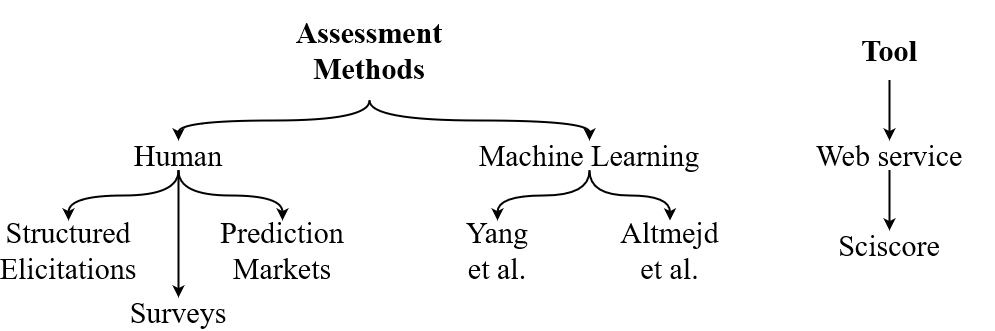
\includegraphics[width=\linewidth]{Figures/assessmens_methods_tree.png}
  \caption{Tree Diagram of the methods and tools found for the assessment of replicability}
\end{figure}


\subsubsection{Human Methods}
The three observed methods used to evaluate reproducibility:
\begin{enumerate}[noitemsep] % [noitemsep] removes whitespace between the items for a compact look
\item Surveys
\item Structured Elicitations
\item Prediction Markets
\end{enumerate}

The Surveys are perhaps the most straightforward out of the three methods. This method consists of giving the reviewers a brief summary of the study and the findings. Each reviewer then makes a prediction for the outcome of the study and the predictions from all the reviewers are then averaged. 

Secondly, Structured Elicitations add more structure to the process. One protocol implemented by the SCORE program when doing structured elicitations, is the IDEA protocol. IDEA stands for INVESTIGATE, DISCUSS, ESTIMATE, AND AGGREGATE. The process has four stages. For the first stage (investigate) the 
reviewers read through the study and make their own judgment on the outcome. The second stage (Discussion) consists of the reviewers sharing their insights and predictions on the study, The third stage (Estimate) consists of making a second individual assessment. The last stage (Aggregate)
consists of averaging the scores of the reviewers. 

Thirdly, Prediction Market is a method in which the reviewer bets on the outcome of a replication study. The reviewers buy and sell shares. These shares pay 1\$ if the study in question is replicated, or 0\$ in case the replication fails. The final market price of a stock (study) is the probability of 
reproducibility. \cite{Dreber2015} used the prediction market to accurately predict 29 out of 41 studies (~71\%) being replicated as part of the Reproducibility Project Psychology \cite{Dreber2015}. 

A recent study attempted to quantify the reproducibility in computing research \cite{Raghupathi2022}. 
They recognised 25 variables related to method, data and experiment, that are the factors influencing the reproducibility of a scientific study. 
Three reproducibility metrics were used namely R1D, R2D and R3D. 
A qualitative survey was conducted in which100 research papers were selected randomly from the International Conference on Information Systems series in the year 2019.
These papers were read several times to determine the values of the 25 variables. 
This study concluded 67 percent of these papers seemed to be reproducible. 
However, none of the 100 research papers addresses all the 25 variables.
Thus, there is a need to prioritise reproducibility while conducing scientific research. 
This study also provides a framework and checklist to assess reproducibility.


The lower the p-value, the greater the statistical significance of the observed difference. A significant value is considered P < 0.05. The P-value can serve as an alternative or complement to pre-selected confidence levels for hypothesis testing. A low p-value shows that the results are replicable.

Moreover, in another study \cite {Gundersen2019}, a call to action for better documentation has been proposed. This paper suggests 20 recommendations, collectively called the "Author Checklist", 
where they provide details along with examples for better documentation to ensure a more reproducible research. The paper includes recommendations for data, source code, AI methods, and experiments.
For example, under experiment recommendations they suggest that hardware specifications documentations should include things such as processor type, number of cores and processors, RAM and disk requirements. 
Under AI methods recommendations, they suggest that the problem being solved by a conceptual AI method should be explicitly described by presenting the context of the problem, outlined conceptually so that anyone can understand the fundamental
concepts and that a pseudocode could be used so that others can understand the details of the work. With more suggestions found in the paper, ultimately the goal is strive for better reproducible research. The authors also argue ten (10) benefits that researchers can enjoy if they were to follow their 
proposed checklist. These include benefits such as increase number of citations to publications, increase the likelihood of being funded for further research, improving the management of your research assets among others. 
Finally, the main objective of this paper is to underscore the benefits of reproducible science and even though it may take more time and effort, but "once you learn it, it becomes a habit" \cite{Baker2016}.






\subsubsection{ML methods}

\cite{Yang2020} designed an artificially intelligent model to measure the replicability of a scientific study. To train and test the model, manually replicated studies were used. It has three stages. First, the nontext data is extracted, for example, author name, graphics, etc. Second, word2vec,a deep neural network was used to quantitively define the relationship between each words in a set of chosen words. Third, the manually replicated outcome is predicted using an ensemble model. The model was able to predict the correct pass or fail outcome for 69 percent of the papers.	Compared to prediction markets and manual survey, this AI model had a higher accuracy of prediction. 


Currently, the industry is in the period that experts have refered to as “The Fourth Industrial Revolution,” also called Industry 4.0. This fact is strongly associated with integrating physical and digital systems of production environments. The integration of these environments allows the collection of a large amount of data collected by different equipment located in various sectors of the factories (Borgi et al., 2017). In addition, new technologies from Industry 4.0 integrate people, machines, and products, enabling a faster and more targeted exchange of information (Rauch et al., in press).

\cite{Altmejd2019} also used machine learning techniques to predict reproducibility. 
Two models were made, namely, a random forest binary classification model and a regression model. 
The regression model predicted the ratio of replication effect size to original effect size. 
This ratio was coined “relative effect size”. 
These models were trained using features from the original experiments from the articles like p-values, effect size, and others similar to Yang's metric-based model. 
The random forest model achieved an accuracy of 0.69 \%. 

A study by \cite{Vijaykumar2019} is focused on assessing replicability in machine learning. Three replication aims were explained in this study. First is test of inconsistency, which investigates if replications reject the original study, using a confidence interval of 95 percent. According to this interval we can see whether the replication has compliance with the original study. 
Second is test a of consistency, assessing statement of successful replication. This aim uses a confidence interval of 90 percent, which is an area around zero. If 90 percent of different estimates lays in this constructed area, they are compatible with the original study. 
Third is about how to get a better accuracy in measuring of prediction, combining replications and constructing meta-data intervals. 
As the measuring method of performance is used R2. 


A framework presented by \cite{Sochat2017} called Singularity Hub, uses the concept of Singularity containers for mobility of compute, and the singularity-python software that has novel metrics for assessing reproducibility of such containers. Scientists and developers are able to package reproducible software because of singularity containers, with automation to such workflows added by Singularity Hub. Their novel metrics, which are based on custom filters of content hashes of container contents, make possible the comparison of an entire container, which includes operating systems, custom softwares, and metadata. The level tests conducted to assess reproducibility, show that utilizing containers can assist researchers in distributing reproducible computing environments with the end goal of making every aspect of computational analyses reproducible and archivable. 







\subsubsection{Web Service}
Based on our reserach ,we found one web service to assess reproducibility. 
It is called Sciscore (\url{https://www.sciscore.com/}). 
The purpose of this tool is to promote reproducibility in scientific research. 
This service receives the user’s manuscript and produces three reports namely Core, MDAR (Materials, Design, Analysis, Reporting) \cite{MDAR2021}, and STAR (structured, transparent, accessible reporting) report to evaluate the quality of the paper. 
The reports follow standards such as NIH, MDAR, and ARRIVE. 
As a scientist author can register using ORCID account and get 10 credits free.
Using each credit, we can create a report. 
If we want to create more reports, it will cost 19 USD for 4 reports. 
To generate a report, we have to mention a few details the of the technical paper like title, author and the method. 
A few minutes after submitting, we get three different reports namely MDAR report, SciScore report, and a csv file that presents the detected tables. 
The SciScore ranges from 0 to 10, 0 indicating low levels of reproducibility and 10 indicating high levels of reproducibility. 

However, it doesn't explain the methods it uses to evaluate reproducibility or to generate these reports which reduces the transparency making this tool less explainable.
Based on our observation, it reads the input text and attempts to understand it.  
For example, it attempts to find if the code is available and extracts the link to access it.
We attempted to submit 10 papers into SciScore portal and generated the reports. 
The results have been presented in the table \ref{table:sciscore_report}.
\begin{table}[!htb]
\caption{SciScore report}
\label{table:sciscore_report}
\begin{tabular}[t]{|p{9cm}|p{3cm}|p{1.3cm}|}
\hline
Paper name & Field & Sciscore \\
\hline
SoftPool++: An Encoder–Decoder Network for Point Cloud Completion & Chemical Engineering & 3\\
High-throughput functional evaluation of human cancer-associated mutations using base editors & Chemical Engineering & n/a\\
Coupling between magnetic order and charge transport in a two-dimensional magnetic semiconductor &  Chemical Engineering & 3 \\
High-throughput functional evaluation of human cancer-associated mutations using base editors &  Biomedical Engineering & 4 \\
A highly photostable and bright green fluorescent protein & Biomedical engineering &  4  \\
Multi-omics single-cell data integration and regulatory inference with graph-linked embedding & Biomedical engineering & 5 \\
High sensitivity isoelectric focusing to establish a signaling biomarker for the diagnosis of human colorectal cancer & Biomedical Engineering & 4\\
Uncovering cancer gene regulation by accurate regulatory network inference from uninformative data	 & Medicine & 3\\
Heterogenous output regression network for direct face alignment & Computer science & 2 \\
Skin feature tracking using deep feature encodings &  Computer science & 2 \\	\hline
\end{tabular}
\end{table}

%Alan
Materials Design Analysis Reporting (MDAR) is a framwork to assess reproducibility in sciscore. 
This framework is work for life science. MDAR investigate in three category: accessibility, 
identification, and characterisation. Accessibility refers to the disclosure of whether and how a
specific Framework element (e.g., material, data, code, or protocols) is accessible, including any
restrictions to that access. Identification refers to the information necessary for unique and
unambiguous designation and provenance of each element (typically this includes a unique persistent identifier).
Characterisation refers to the minimum description of the item which is relevant for interpretation and replication.


\subsubsection{Accuracy of methods to assess reproducibility}
\begin{table}[!ht]
    \centering
    \caption{Accuracy of methods to assess reproducibility}
    \label{table:accuracy_assessment_methods}
    \begin{tabular}{|l|l|}
    \hline
        Method & Accuracy \\ \hline
        Yang et al.  & 71\% \\ \hline
        Altmejd et al.  & 69\% \\ \hline
        Prediciton Markets  & 69\% \\ \hline
    \end{tabular}
\newline\newline \centering * Methods should be directly compared, because their the training samples differ
\end{table}

We have learned about the problem of reproducibility and the recent efforts to strengthen science by means of more stringent measures on reproducibility. 
Road to reproducibility will require the combined efforts of human evaluation and computational algorithms. 
Making a web service to assess reproducibility is a viable solution to contribute to the scientific community. 
The current drawback of methods that require human intervention are cost and time. 
Machine learning algorithms, if proven accurate, can save researchers significant time and money when preparing their literature review. 
In addition, a reproducibility tool could validate or discard published results and thus enhance the current level of knowledge in any given field. 


\subsection{Metrics to assess reproducibility}
There are a variety of metrics used to assess reproducibility. It can be majorly categorised into two parts - survey and machine learning. We have discussed about the survey and the machine learning approaches to assess reproducibility in the previous section. The figure \ref{fig:tree_diagram_metrics} represents a tree diagram of different types of metrics to assess reproducibility. 

A study by \cite{Gundersen2019} quantified reproducibility naming the metrics $R1$, $R2$ and $R3$. This metric measures how well the different sections like Methods, Data and Experiment, of a technical paper are documented for experiment $e$. The factors are Methods, Data and Experiment which are defined by 16 boolean variables explained in the Table \ref{table:variables_16} The metrics are defined as
\begin{align}
	R1D(e)&= (\delta_1 Method(e) +\delta_2 Data(e) +\delta_3 Exp(e))/(\delta_1+\delta_2+\delta_3)\\
	R2D(e)&= (\delta_1 Method(e) +\delta_2 Data(e))/(\delta_1+\delta_2)\\
	R2D(e)&= \delta_1 Method(e), 
\end{align}
where $\delta_1$, $\delta_2$, and $\delta_3$ are the weights of the factors Method, Data and Experiment respectively. 
$Method(e)$, $Data(e)$, and $Exp(e)$ are defined as weighted sums of the true values of the variables listed under the three factors Method, Data and Experiment respectively. 
For example, the value of $Data(e)$ is the summation of the truth values for wheather the training validation and test dataset, and the results are shared for $e$. Different weights could be assigned to different factors. 
\begin{table}[H]
\caption{Variables to measure reproducibility}
\centering
\label{table:variables_16}
\begin{tabular}[t]{|p{2cm}|p{2cm}|p{9cm}|}
\hline
Factors & Methods & Description \\
\hline
Method & Problem & Is there an explicit mention of the problem the research seeks to solve? \\
Method & Objective & Is the research objective explicitly mentioned? \\
Method &  Research method & Is there an explicit mention of the research method used (empirical, theoretical)? \\
Method &  Research question& Is there an explicit mention of the research question(s) addressed? \\
 Method & Pseudocode &  Is the AI method described using pseudocode?  \\
Method & Hypothesis & Is there an explicit mention of the hypotheses being investigated? \\
Method & Prediction &  Is there an explicit mention of predictions related to the hypotheses? \\
Method & Experimental setup & Experiment setup Are the variable settings shared, such as hyperparameters? \\
Data & Training data & Training data Is the training set shared? \\
Data & Validation data & Validation data Is the validation set shared? \\
Data & Test data & Test data Is the test set shared? \\
Data & Results & Are the relevant intermediate and final results output by the AI program shared? \\
Experiment & Method source code & Method source code Is the AI system code available open source? \\
Experiment & Experiment source code & Experiment source code Is the experiment code available open source? \\
Experiment & Software dependencies & Software dependencies Are software dependencies specified? \\
Experiment & Hardware & Hardware Is the hardware used for conducting the experiment specified?\\ \hline
\end{tabular}
\end{table}

A recent study by \cite{Raghupathi2022} conducted a survey on computing reproducibility and used the same metrics $R1$, $R2$ and $R3$. However, for they have added a few more variables making it total $25$ variables to assess reproducibility. The table \ref{table:variables_25} in the appendix \ref{appendix:tables_for_metrics_to_assess_reproducibility} presents the variables with descriptions. These $25$ variables are defined to measure computational reproducibility. 

Yang et al. designed a machine learning algorithm that can test reproducibility. The metrics used were accuracy score and Top-K precision score. These scores measure the predictive accuracy. These scores depend on the training dataset. The model is trained by giving on a dataset which has multiple papers manually surveyed for reproducibility. 

\begin{figure}[!hbt] 
\centering
  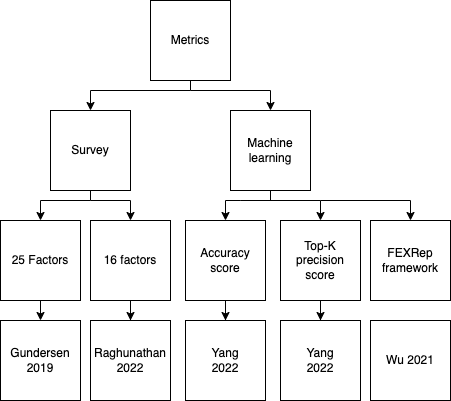
\includegraphics[scale=0.5]{Reproducibility_metrics.png}
  \caption{Tree Diagram of the metrics used for the assessment of reproducibility}
  \label{fig:tree_diagram_metrics}
  \end{figure}

FEXRep (Feature EXtraction framework for Replicability prediction) is a framework designed to assess reproducibility using ML \cite{Wu2021PredictingTR}. 
This framework is able to extract bibliometrics, venue, author, statistic and semantic features from SBS papers. Firstly from a paper, 
are directly extracted raw information including DOI, authors and citations, secondly are derived numerical values for building feature vectors. 
The framework FEXRep is modular, scalable, and customisable. It allows to add new extractors and existing ones can be updated to give a better performance.
Then extraction results were used to predict reproducibility. By doing statistical correlation and feature analysis, from 139 papers were selected 9 features,
which were the most important. 
FEXRep framework can automatically extract 41 features from research papers. All the 41 features have been explained in the appendix \ref{appendix:tables_for_metrics_to_assess_reproducibility} in the table \ref{table:variables_41_FEXREP}.The main goal of creating the framework was to extract features, which could be used for reproducibility prediction. The table \ref{table:metrics_comparision} represents a comparison between the different types of metrics used to assess reproducibility.

\begin{table}[!htb]
\caption{Comparison of metrics to assess reproducibility}\
\label{table:metrics_comparision}
\begin{tabular}[t]{|p{2cm}|p{2cm}|p{1cm}|p{3cm}|p{2cm}|}
\hline
Metric name & Author      & Year                     & Type (survery/ML) & Number of factors      \\ \hline
R1, R2, R3  & Gundursen   & 2019 & survey             & 16 \\ \hline
R1, R2, R3  & Raghupathi & 2022 & survey             & 25 \\ \hline
FEXRep & Wu & 2021 & ML             & 41 \\ \hline
\end{tabular}
\end{table}

\subsection{Studies that attempt to assess reproducibility}
%%%%%%%%%%%%%%%%%%
% Google scholar (Huy)
% Review paper 1
There are many articles about assessment of reproducibility of scientific researches.
In \cite{iqbal2016reproducible}, they assess the status of reproducibility and transparency in 441 biomedical journal articles published in 2000-2014. 
Only 1 study provided a full protocol and none made all raw data directly available. 
The majority of studies did not mention anything about funding or conflicts of interest. 
Their empirical evaluation shows that the published biomedical literature lacks transparency in important dimensions. 
The majority of papers claimed to present some novel discoveries, however, they suspect that very few papers truly have totally, disruptively innovative findings.\\
The indicators assessed in this paper include: protocol availability, dataset availability,  funding, and replication.\\
To assess protocol availability, they reviewed the eligible papers for any mention of the protocol, possible hyperlink, or reference to the source for available protocol.\\
To assess dataset availability, articles were scrutinised for any mention of access to the datasets that stand behind the analyses presented in the paper. If studies had datasets, they recorded whether the available datasets cover all or part of the presented analyses.\\
The indicators assessed by the authors are given
\href{https://www.dropbox.com/home/%5BGroup%201%5DScientific%20Information%20Share/literature_review_Group/Literature%20review%20on%20assessments%20of%20reproducibility/Reproducibility%20data?preview=Paper+1+result.xlsx}{here}.

% Review paper 2
In \cite{Stagge2019Assessing}, they developed a survey tool to assess the availability of digital research artifacts published alongside peer-reviewed journal articles (e.g. data, models, code, directions for use) and reproducibility of article results.
They used the tool to assess 360 of the 1,989 articles published by six hydrology and water resources journals in 2017.
They estimated that results might be reproduced for only 0.6\% to 6.8\% of all 1,989 articles.
The survey tool identified key bottlenecks to making work more reproducible, include: only some digital artifacts available (44\% of articles), no directions (89\%), or all artefacts available but results not reproducible (5\%).
The tool can help authors, journals, funders, and institutions to self-assess manuscripts, provide feedback to improve reproducibility, and recognise and reward reproducible articles as examples for others.
The 15-questions survey tool used in this paper is available as Google Form
\href{https://docs.google.com/forms/d/e/1FAIpQLSdWvcUUjUT6k2sBRe9pIBca_BPUdE8kMmyUGvCZkWmnq-UDvQ/viewform}{here}.\\
The survey results completed by authors are available
\href{https://www.dropbox.com/home/\%5BGroup\%201\%5DScientific\%20Information\%20Share/literature_review_Group/Literature\%20review\%20on\%20assessments\%20of\%20reproducibility/Reproducibility\%20data?preview=Paper+2+result.xlsx}{here}.

%Omar-SpinBEC-
\section{Description of Our Web Service and Its Features}

In this section we describe the features of our web service and its basic features. Our web service at it most basic allows a user to upload a PDF file and outputs extracted information from that file. In more details, when you go to our web service the user is prompted 
to upload a PDF file. We have written the code such that when you upload a file, the service checks that the file being attempted to upload is indeed in PDF (Portable Document Format), i.e. a file with a .pdf extension. Any file that is not a PDF file will cause an error to be shown on the screen. 
After a successful upload, the file is converted to text so that important information is extracted. You can find further information on how our web service uses tools such as GROBID and pdftotext below convert the PDF file into text. 
The information we can extract include: article's name, author's name, URLs in the article, and number of references. Finally, the web service is being hosted on an NGINX server and we use Flask framework this web service. In addition, a Docker container is used to ensure that our web service can run on different operating systems. 

But how did we deploy all of this? We deployed using a virtual machine. The service provider that we chose was Linode becuase it is very user  friendly. Linode offered virtual machines with pre-installed software that can support very popular applications. In order to deploy our application, we used Linode's Docker virtual machine 
because no installation or set up was required as the virtual machine was already pre-installed.
Then, we cloned our reprodm repository to our virtual machine and ran the command to build the container. Furthermore, the application  was up and running in less than five minutes. To test it, we also briefly deployed and ran it on Nordling Lab's Canada server. To further test, several students also ran the appiication locally in their 
computers. To find out further details about how our application  is updated kindly visit the following URL and scroll to the last section of the README file in "flask{\_}docker": https://bitbucket.org/nordlinglab/nordlinglab-re\\prodm/src/master/flask{\_}docker/README.md.


% Web of Science (Thanh)
Currently, a key component of scientific communication is sufficient information for other researchers in the field to reproduce published findings. For computational and data-enabled research, this has often been interpreted to mean 
making available the raw data from which results were generated, the computer code that generated the findings, and any additional information needed such as workflows and input parameters. Many journals are revising author guidelines to include 
data and code availability. In \cite{stodden2018empirical}, the author evaluates the effectiveness of journal policy that requires the data and code necessary for reproducibility to be made available postpublication by the authors upon request.
204 scientific papers published in the journal Science were chosen, in which 44\% of chosen study and were able to reproduce the findings for 26\%. The paper presented this policy—author remission of data and code postpublication upon request—an improvement over no policy, but currently insufficient for reproducibility. In this paper, survey methods, replication and evaluation methods were applied. All of material of the paper was updated in \href{https://github.com/ReproducibilityInPublishing/Science-2018}{here}, including the survey, coding, and data.

The demand for reproducible research is on the rise in disciplines concerned with data analysis and computational methods. In \cite{nust2018reproducible}, the author reviewed current recommendations for reproducible research and translated them into criteria for assessing the reproducibility of articles in the field of geographic information science (GIScience). Using this criterion, they assessed a sample of GIScience studies from the Association of Geographic Information Laboratories in Europe (AGILE) conference series, and they also collected feedback about the assessment from the study authors. Results from the author's feedback indicate that although authors support the concept of performing reproducible research, the incentives for doing this in practice are too small. Therefore, the author proposed concrete actions for individual researchers and the GIScience conference series to improve transparency and reproducibility. The available data were published in \href{https://github.com/nuest/reproducible-research-and-giscience}{this}, 
including the survey, programming , and evaluate data.

% Scopus (Kung)
In \cite{PAGE20188}, they explored whether the use of reproducible research practices was associated with an Systematic Review (SR) being a Cochrane review, as well as with the reported use of the Preferred Reporting Items for Systematic Reviews and Meta-Analyses statement, and they evaluated 110 SRs of therapeutic interventions, 78 (71\%) of which were non-Cochrane SRs. Across the SRs, there were 2,139 meta-analytic effects (including subgroup meta-analytic effects and sensitivity analyses), 1,551 (73\%) of which were reported in sufficient detail to recreate them. And finally Reproducible research practices are underused in SRs of biomedical interventions. Adoption of such practices facilitates identification of errors and allows the SR data to help us  reanalyzed.

Besides, we can find many articles talking about the string assessment of reproducibility. Furthermore, in the article \cite{MAHMOOD2018148}, they investigate the replication of defect prediction studies and identify the characteristics of replicated studies, and then  they further assess how defect prediction replications are performed and the consistency of replication findings. So that Only 13 (6\%) of the 208 studies are replicated. Replication seems related to original papers appearing in the Transactions of Software Engineering (TSE) journal. The number of citations an original paper had been also an indicator of replications. In addition, studies conducted using closed source data seems to have more replications than those based on open source data. Where a paper has been replicated, 11 (38\%) out of 29 studies revealed different results to the original study. Finally, in this article, Very few defect prediction studies are replicated. The lack of replication means that it remains unclear how reliable defect prediction is. And confirm practical steps for improving the state of replication.

% Scopus (Alvin)
Using the data analysis method, Once all discrepancies between data collectors had been resolved, the data set for all included SRs was exported from DistillerSR into Microsoft Excel, where data was cleaned (i.e., invalid characters were removed and text data were converted to numeric where appropriate). Data for some items collected in the previous study. on general characteristics of the SRs (e.g., clinical focus, country of corresponding author) were merged with the current data set. We summarized data as frequency and percentage for categorical items and median and interquartile range (IQR) for continuous items. We analyzed characteristics of all SRs and of SRs categorized as Cochrane or non-Cochrane. We explored whether use of reproducible research practices was associated with an SR being a Cochrane review and, in a post-hoc analysis, with self-reported use of the PRISMA statement.

The scientific community and decision-makers are increasingly concerned about transparency and reproducibility of epide-miologic studies using longitudinal healthcare databases. We explored the extent to which published pharmacoepidemio-logic studies using commercially available databases could be reproduced by other investigators.Full reproducibility in healthcare database studies occurs when independent investigators are able to apply the same design and analytic choices to the same source data, and are able to obtain the same analytic population and estimated measures of associa-tion (or at least a near exact reproduction). The scientific com-munity as a whole would benefit and the credibility of healthcare database studies would increase if greater effort were directed toward ensuring that public reporting for database studies con-tained sufficient detail to allow full reproduction. Without repro-duction there can be no replication and without replication there can be little trust in our research output.

Metrics to quantify reproducibility
In order to quantify the reproducibility of studies, they focused on two categories: (1) reproduction of the patient cohort and (2) reproduction of the statistical analysis. For the former, they compared population descriptive measures between our reproduction and the original published study; for the latter, they compared measures of association. 
\begin{figure}[h]
    \centering
    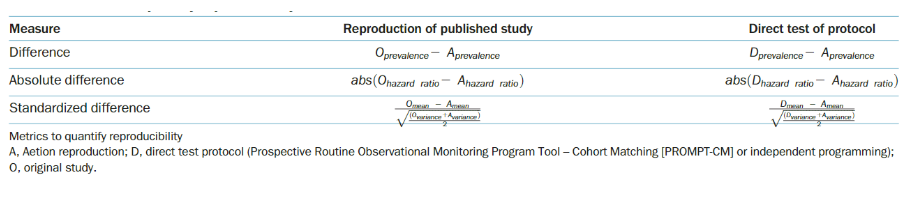
\includegraphics[width = 14cm]{metrics.png}
    \caption{Metrics }
    \label{fig:metric}
\end{figure}

All papers assessed by these 6 articles are given
\href{https://www.dropbox.com/home/NordlingLab_Course_ScientificInformation/Team_Freshman/Literature\%20review\%20on\%20assessments\%20of\%20reproducibility}{here}. Also, the search string is mentioned in the appendix \ref{appendix:search_strings}.






%Omar-SpinBEC-
\subsection{Features of our webservice}

In this section we describe the features of our web service and its basic features. Our web service at it most basic allows a user to upload a PDF file and outputs extracted information from that file. In more details, when you go to our web service the user is prompted 
to upload a PDF file. We have written the code such that when you upload a file, the service checks that the file being attempted to upload is indeed in PDF (Portable Document Format), i.e. a file with a .pdf extension. Any file that is not a PDF file will cause an error to be shown on the screen. 
After a successful upload, the file is converted to text so that important information is extracted. You can find further information on how our web service uses tools such as GROBID and pdftotext below convert the PDF file into text. 
The information we can extract include: article's name, author's name, URLs in the article, and number of references. Finally, the web service is being hosted on an NGINX server and we use Flask framework this web service. In addition, a Docker container is used to ensure that our web service can run on different operating systems. 


%Omar and Alan-SpinBEC-WebService set up

%Omar
We initially set up the web service in a manual way. We had to download, install and set up each code, dependencies, and tools individually. The folder flask{\_}webpage contains all the files for the relevant set up we made. Next, we restructured the application to be run on a docker container. The reason for this is that it facilitates the set-up process for future builds.
In addition, the website  was developed using a micro framework. However, this framework is not as complete as Django, but Flask is able to provide the main functionalities for any new users. 

We used a couple tools to achieve the set up of our web service. First, as mentioned before, we used a flask micro framework for the backend. Furthermore, we used html and a some CSS Bootstrap templates for the frontend. Moreover, we used docker for deployment and Nginx for load balancing. The sequential working of the web service is presented in the figure \ref{fig:uml_sequence_diagram}.

\begin{figure}[!hbt]
\centering
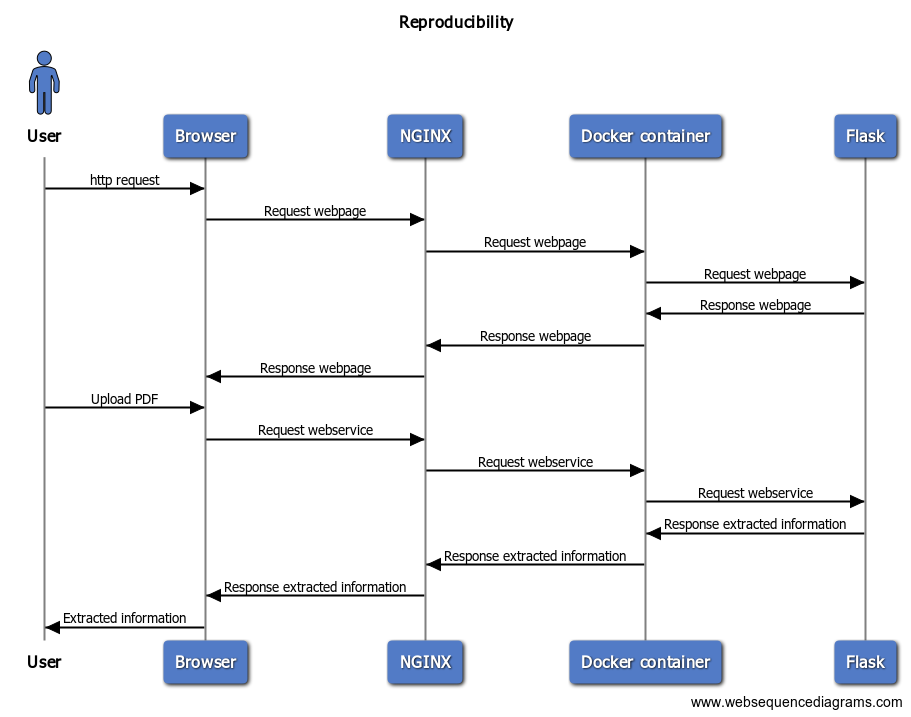
\includegraphics[scale=0.4]{uml_sequence_diagram}
\caption{UML sequence diagram of our web service}
\label{fig:uml_sequence_diagram}
\end{figure}








\subsubsection{Core features of our product}

\begin{itemize}
	 \item Implement the top three PDF to text open source libraries.
	\item Implement the GROBID open source library for conversion to XML and extraction of citation metrics, see \url{https://github.com/kermitt2/grobid}.
	\item Implement all open source libraries for extracting reproducibility metrics, such as FEXREP.
	\item Visualise the results: \subitem PDF with the extracted areas highlighted using different colors. \subitem Table of all reproducibility metrics and numbers for the uploaded article with the min, median, mean, and max for the database of assessed articles.
	\item Easy download of a csv with the reproducibility metrics, a txt (UTF8) file with the extracted text, and xml file of the pdf.
	\item It should contain a database of all articles that previously have been assessed for reproducibility.
\end{itemize}

The 

\subsubsection{Structure and function of the product}
% Freshman - Huy
\begin{figure}[!hbt]
\centering
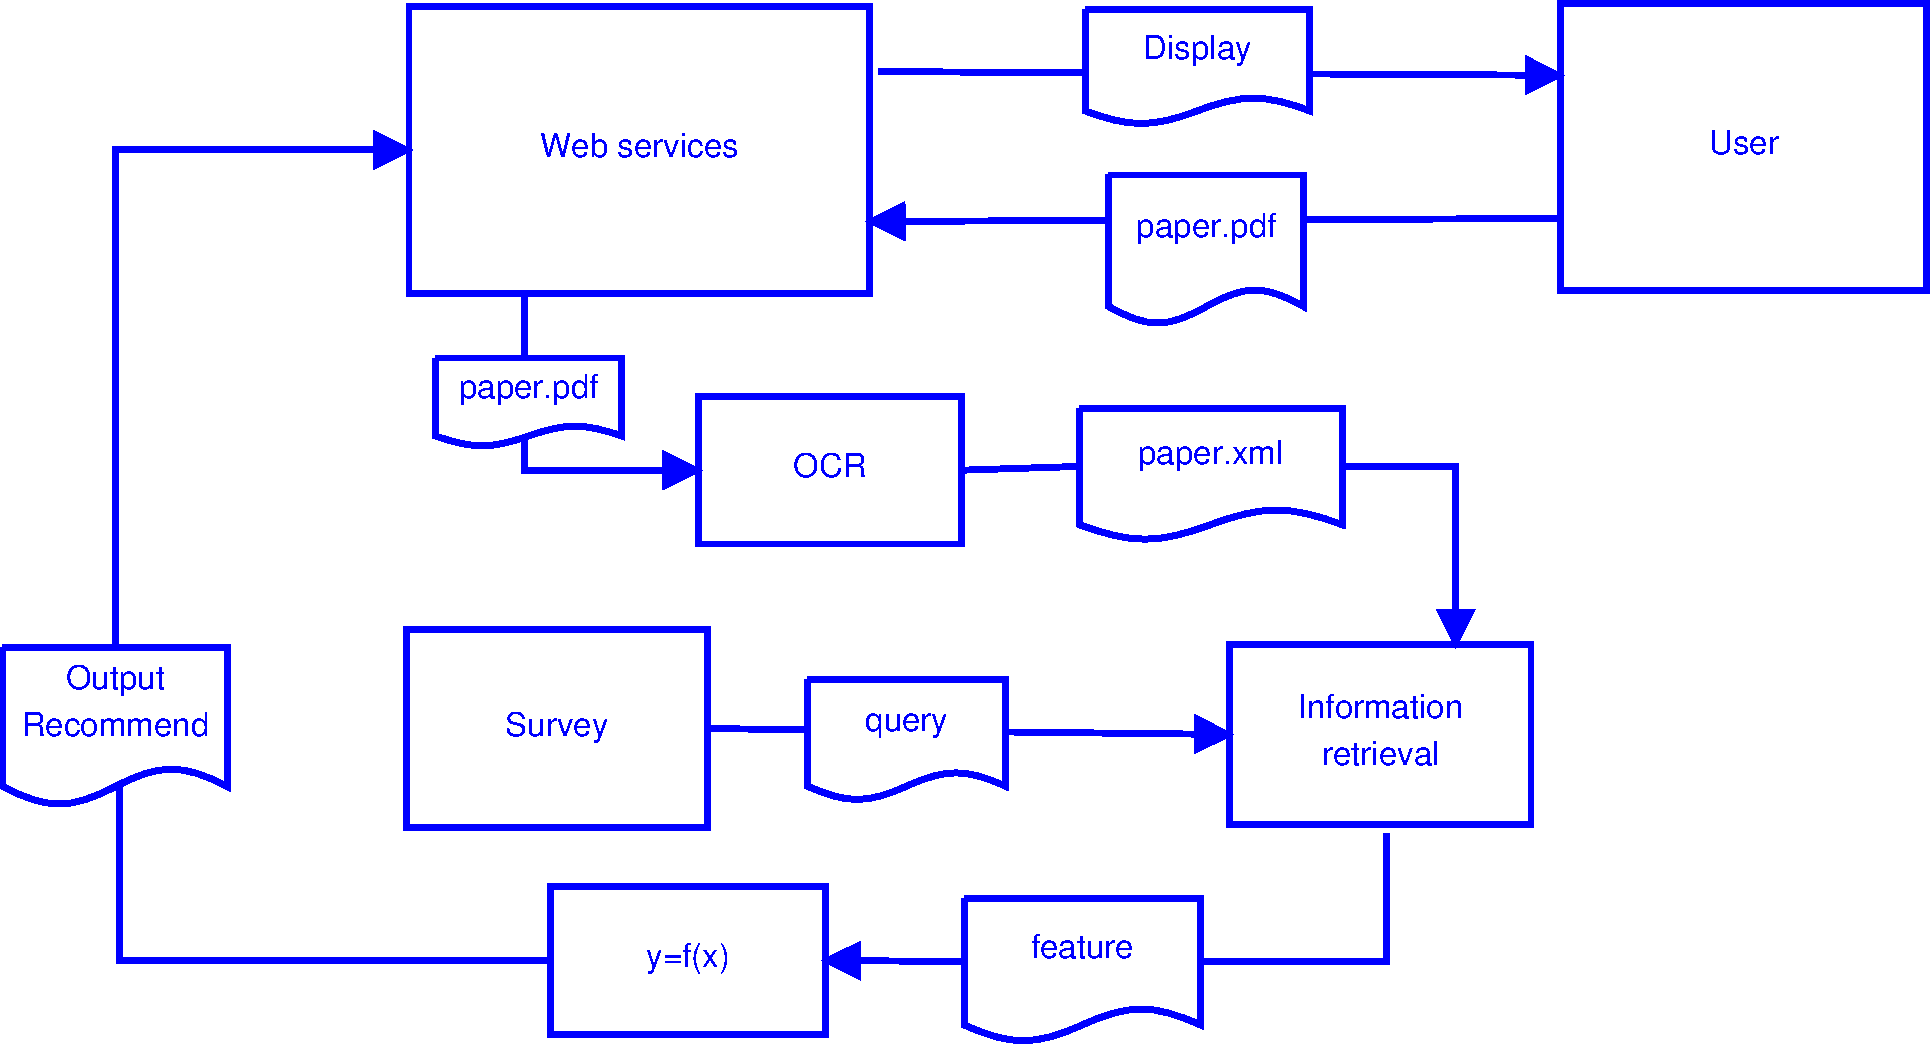
\includegraphics[scale=0.4]{productStructure}
\caption{Overview of product's structure}
\label{fig:productStructure}
\end{figure}
Figure \ref{fig:productStructure} shows the overview of structure of our product.
The web service is the interface between the software and user.
Users can input the paper they want to assess reproducibility to the web service.\\
An optical character recognition block is developed to convert \textbf{PDF} format files to \textbf{XML} format.\\
From the tools and methods to assess reproducibility identified from the literature review, we build the queries to search for the relevant information in the paper.
The output of the Information Retrieval block is the quantified features relevant to reproducibility of the paper.
A function $y=f(x)$ that describe the relationship between input (features) and output (reproducibility) is then designed.\\
If we don't know exactly the function $f(x)$, we can apply machine learning methods to approximate this function. In order to do that, we need a reliable database that contains papers with features and reproducibility metric after quantification process.\\
The output of our software is the reproducibility of the paper, and it is printed to the web services. If the users' paper is not reproducible, our software will print some recommendation for them to improve the reproducibility of their papers. The use case diagram of the web service is presented in the figure \ref{fig:uml_use_case_diagram}.\\

\begin{figure}[!hbt]
\centering
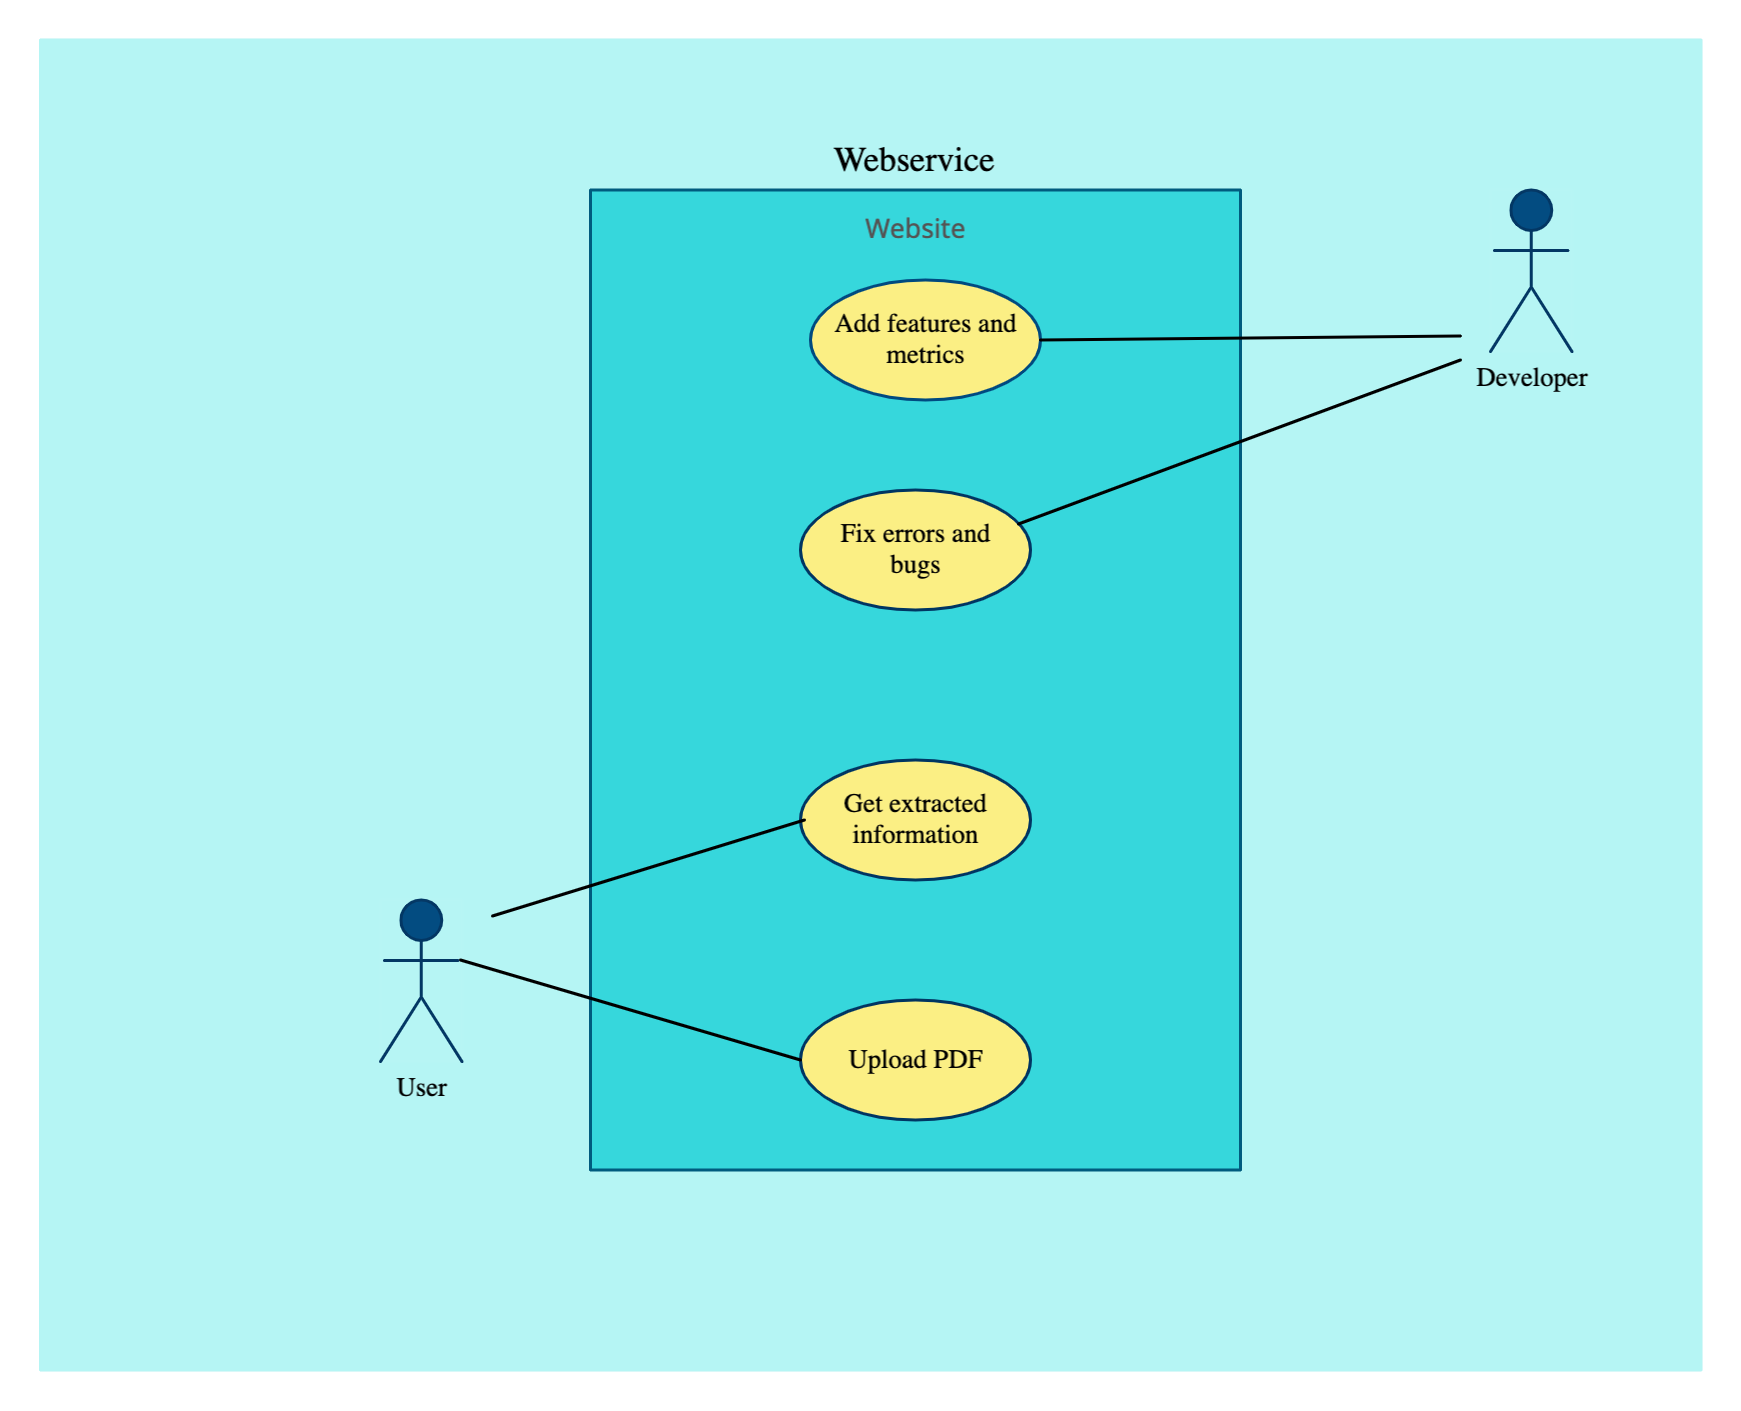
\includegraphics[scale=0.2]{uml_use_case_diagram}
\caption{Use case diagram of the web service}
\label{fig:uml_use_case_diagram}
\end{figure}


% Freshman - Kung
From user's perspective these functions can make our product more user-friendly
\begin{enumerate}[noitemsep] % [noitemsep] removes whitespace between the items for a compact look
\item Simple and clear user interface and fool-proof mechanism
\item History storage function
\item Plug-ins can be added
\item Graphical function menu
\item The homepage recommends related types of articles
\item Very low memory, low CPU usage, good performance, and rich modules
\item Supports computer and mobile apps and replaces accounts with codes for one-click connection
\end{enumerate}





\subsection{A tool for convert PDF to XML: GROBID}
GROBID (or Grobid, but not GroBid nor GroBiD) means GeneRation Of BIbliographic Data.
GROBID is a machine learning library for extracting, parsing and re-structuring raw documents such as PDF into structured XML/TEI encoded documents with a particular focus on technical and scientific publications. First developments started in 2008 as a hobby. In 2011 the tool has been made available in open source. Work on GROBID has been steady as side project since the beginning and is expected to continue as such.
GROBID includes batch processing, a comprehensive web service API, a JAVA API, a docker container, a relatively generic evaluation framework (precision, recall, n-fold cross-valiation, etc.) and the semi-automatic generation of training data.

In a complete PDF processing, GROBID manages 55 final labels used to build relatively fine-grained structures, from traditional publication metadata (title, author first/last/middlenames, affiliation types, detailed address, journal, volume, issue, pages, doi, pmid, etc.) to full text structures (section title, paragraph, reference markers, head/foot notes, figure headers, etc.).

GROBID can be considered as production ready. Deployments in production includes ResearchGate, HAL Research Archive, the European Patent Office, INIST-CNRS, Mendeley, CERN (Invenio), Internet Archive, and many others.
The key aspects of GROBID are the following ones:

Written in Java, with JNI call to native CRF libraries and/or Deep Learning libraries via Python JNI bridge.
Speed - on low profile Linux machine (8 threads): header extraction from 4000 PDF in 2 minutes (36 PDF per second with the RESTful API), parsing of 3500 references in 4 seconds, full processing of 4000 PDF (full body, header and reference, structured) in 26 minutes (around 2.5 PDF per second).
Scalability and robustness: We have been able recently to run the complete fulltext processing at around 10.6 PDF per second (around 915,000 PDF per day, around 20M pages per day) during one week on one 16 CPU machine (16 threads, 32GB RAM, no SDD, articles from mainstream publishers), see here (11.3M PDF were processed in 6 days by 2 servers without crash).
Lazy loading of models and resources. Depending on the selected process, only the required data are loaded in memory. For instance, extracting only metadata header from a PDF requires less than 2 GB memory in a multithreading usage, extracting citations uses around 3GB and extracting all the PDF structures around 4GB.
Robust and fast PDF processing with pdfalto, based on xpdf, and dedicated post-processing.
Modular and reusable machine learning models for sequence labelling. The default extractions are based on Linear Chain Conditional Random Fields, with the possibility to use various Deep Learning architectures for sequence labelling (including ELMo and BERT-CRF). The specialized sequence labelling models are cascaded to build a complete (hierarchical) document structure.
Full encoding in TEI, both for the training corpus and the parsed results.
Optional consolidation of extracted bibliographical data via online call to biblio-glutton or the CrossRef REST API, export to OpenURL, BibTeX, etc. for easier integration into Digital Library environments. For scalability, reliability and accuracy, we recommend to use biblio-glutton when possible.
Rich bibliographical processing: fine grained parsing of author names, dates, affiliations, addresses, etc. but also for instance quite reliable automatic attachment of affiliations and emails to authors.
Automatic generation of pre-annotated training data from new PDF documents based on current models, for supporting semi-automatic training data generation.
Support for CJK and Arabic languages based on customized Lucene analyzers provided by WIPO.
PDF coordinates for extracted information, allowing to create "augmented" interactive PDF. The figure \ref{fig:uml_class_diagram} presents the UML class diagram of the webservice. 

\begin{figure}[!hbt]
\centering
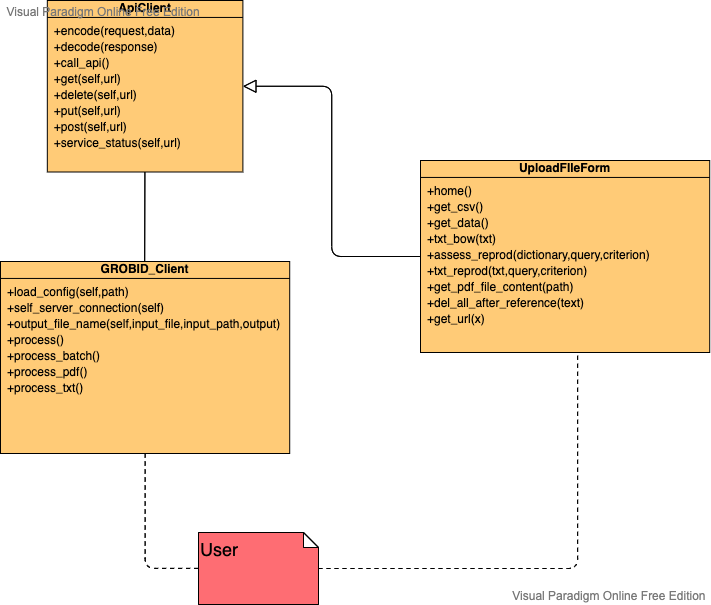
\includegraphics[scale=0.4]{uml_class_diagram}
\caption{Class diagram of the web serivce}
\label{fig:uml_class_diagram}
\end{figure}


\subsubsection{Setting up GROBID}

Setting up GROBID:

Obtain the latest version via GitHub, Docker or simply pull the latest release by

\$ wget https://github.com/kermitt2/grobid/archive/0.5.5.zip \&\& unzip 0.5.5.zip

Build GROBID using gradle\$

\$./gradlew clean install\$

Run the REST service

\$ ./gradlew run\$

which makes the GROBID service available on port 8070.

\subsubsection{Using GROBID}
GROBID offers a web user interface to interactively submit pdfs. In addition, you can invoke these services via a REST API. We discuss both how to use the web user interface and use the REST API, via curl and REST clients from GROBID.

To use the web interface, open http://localhost:8070 in your browser.

You can decide whether you want to retrieve the paper’s header (Process Header Document) get the paper’s entire full text (Process Fulltext Document) or obtain just the paper’s references (Process All References)

After completing generating the xml document, you can either inspect the document or download it.

This document contains already a lot of information about the publication! So what is TEI? TEI stands for Text Encoding Initiative. As its name already hints, TEI is a standard guiding how to encode digital texts. I’ll cover parsing TEI files in another post.

\subsubsection{Using GROBID with Docker}
Docker is an open-source project that automates the deployment of applications inside software containers. The documentation on how to install it and start using it can be found here.
GROBID can be instantiated and run using Docker. For convenience, we provide two docker images:
a lightweight image with only CRF models: this image offers best performance in term of runtime and memory usage, as well as limiting the size of the image. The image information can be found here.
A full image able to run both CRF and Deep Learning models: this image includes all the required python and TensorFlow libraries, GPU support and all DL model resources. It can provide slighly more accurate results, but at the cost of much slower runtime and higher memory usage. The image is also considerably larger (python and tensorflow libraries taking more than $2$ GB and pre-loaded embeddings around $5$ GB).

We assume in the following that docker is installed and working on your system. Note that the default memory available for your container might need to be increased for using all the available GROBID services, in particular on macros, see the Troubleshooting section below.
CRF-only image
The process for retrieving and running the image is as follow:

Pull the image from docker HUB (Check the latest version number):
\begin{verbatim}
> docker pull lfoppiano grobid:$ {latest\_grobid\_version}
Run the container:
> docker run -t --rm --init -p 8070:8070 lfoppiano/grobid:$ {latest\_grobid\_version}

Latest version:

> docker run -t --rm --init -p 8070:8070 lfoppiano/grobid:0.7.1
Note the default version is running on port 8070, however it can be mapped 
on the more traditional port 8080 of your host with the following command:

> docker run -t --rm --init -p 8080:8070 -p 8081:8071 
lfoppiano/grobid:\${latest_grobid_version}
\end{verbatim}
Access the service: - open the browser at the address \url{http://localhost:8080} - the health check will be accessible at the address \url{http://localhost:8081}.

GROBID web services are then available as described in the service documentation.

\subsubsection{Extracting data from GROBID cloud using grobid-tei-xml 0.1.3}

This is a simple python library for parsing the TEI-XML structured documents returned by GROBID,
a machine learning tool for extracting text and bibliographic metadata from research article PDFs.

TEI-XML is a standard format, and there exist other libraries to parse entire documents and work with annotated text.
This library is focused specifically on extracting "header" metadata from document (eg, title, authors, journal name, volume, issue),
content in flattened text form (full abstract and body text as single strings,
for things like search indexing), and structured citation metadata.

Grobid{\_}tei{\_}xml works with Python 3, using only the standard library.
It does not talk to the GROBID HTTP API or read files off disk on it's own, but see examples below.
The library is packaged on pypi.org.

Install using pip, usually within a virtualenv:

pip install grobid{\_}tei{\_}xml

The main entry points are the functions process{\_}document{\_}xml(xml{\_}text) and process{\_}citationxml(xml{\_}text)
(or process{\_}citation{\_}list{\_}xml(xml{\_}text) for multiple citations), which return python dataclass objects.
The helper method .to{\_}dict() can be useful for, eg, serializing these objects to JSON.

Usage Examples:

Use requests to download a PDF from the web, submit to GROBID (via HTTP API), parse the TEI-XML
response with grobid{\_}tei{\_}xml, and print some metadata fields.


%\begin{figure}[!htb]
%    \centering
%    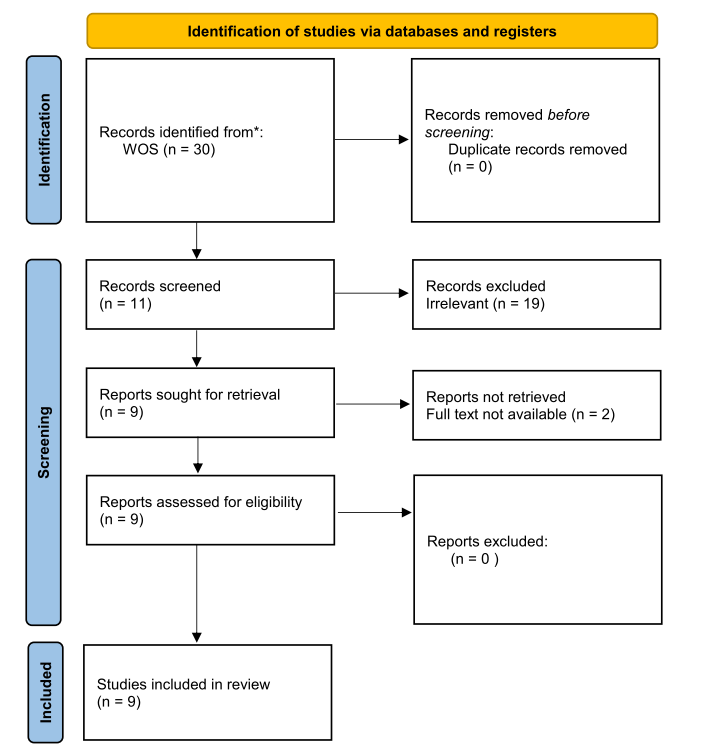
\includegraphics[width = 12cm]{PRISMA_metrics.png}
%    \caption{PRISMA flow chart of metrics}
%    \label{fig:Chart}
%\end{figure}

\section{Project Management}
%Jirka
In this section we describe the project management strategies used to design and deploy the web service. The individual tasks were divided between the three teams. Two of the teams had five members, and one team had four members. Furthermore, the tasks were divided into so-called sprints, where each team was given a certain number of tasks per sprint. These were to be completed every Thursday (with one exception, when we were given two weeks to complete the sprint), where the lesson was presented during the lesson and the feedback from the professor took place. During these sprints each team were tasked to have a scrum meeting, which means to have a short facetime meeting every day (except weekends) within each team. In the teams, a so-called scrum master was elected for each week, whose task was to lead the meeting. The main questions that should be asked and answered during each meeting are: "What did you accomplish yesterday? What will you do today? What problems do you need help with from the team or external parties?" The scrum master was responsible for completing the tasks in the sprint. During each lesson on Thursday, there was always some time during which we evaluated the sprints and scrum meetings from the past week within the team. We should always answer the questions: "What was working? What did not work? What will help us do better in the future?" Each member of the team was asked to give their answer. The answers were then written down. 

Here are some answers to each question across the teams:
\begin{itemize}
\item "What was working?" 
	\subitem "People were responsible for completing their tasks." 
	\subitem "Collaborated with other teams to promote cooperation" 
	\subitem "Class sprint seemed more effective to get tasks done and we work well based on your competencies." 
	\subitem "Easy to break down the tasks and we knew how to get it done" 
\item "What did not work?"  
	\subitem "We had some commit and merge issues with slowed down our progress." 
	\subitem "Some tasks were not finished" 
	\subitem "No new tasks added to flying donut"  
	\subitem "Problems with Latex and Source tree"  
	\subitem "Time conflicts for daily scrums"   
\item  "How to make next sprint successful?" 
\subitem "1 physical meeting at the end" 
\subitem "Give more feedbacks in the meeting" 
\subitem "Make tasks independent" 
\subitem "Point out problem when it occurs, not when it’s too late."
\end{itemize}

 We also learned about waterfall, which is helpful during project management. The waterfall is one of the most popular methodologies in the field of modern software development. This system checks that one phase of product formation is fully completed before the next begins, with no overlap between the individual phases. The timing and budget are fully set. The classical form of the model consists of successive phases in the following order: Requirements analysis Design Development Testing Operations (Maintenance) Teams were discussing about waterfall’s advantages and disadvantages.  

Some of the advantages are: 
\begin{itemize}	
\item Requirements are clear and are not changed throughout the entire project development.
 \item Careful planning helps reduce the incidence of problems throughout the project. 
 \item It provides easy control and transparency for the customer due to a strict reporting system    
 \end{itemize}
 Disadvantages are: 
 \begin{itemize}	
\item	 Requirements must be known before development starts, which delays the project start.
\item	 Strict rules in adjusting the order of product stages make it very difficult, or even impossible, to make any changes.
\item Strict management and monitoring are needed to make sure the project hit the deadlines.  
\item	 The client does not have the opportunity to get acquainted with the system in advance, so he does not see the product until the moment of its completion.
\end{itemize}

\subsection{User stories}
%Freshman - Tho & Alvin - User stoies:
To develop a product that can access reproducibility data from publications we define user stories:\\
%Tho & Alvin
Within the fifty-four user stories of the class, the Freshman team performs a meta-analyze method to evaluate the stories. Indeed, the evaluation process contains four steps. Firstly, all stories are categorized into eight main ideas which have the same topic like the same AI web service or the same assessment the reproducibility...Secondly, the specific ideals are created by the combination of the main ideal and initial user stories. That specific ideals contain the ideal per the main ideal. In the third step, the two groups of sub-user story built by restructuring the similar ideal of the main and specific ideal. Lastly, the final six user stories were released with the merge of the above two sub-story as below:

1. As a student, I need a web service that can use a database to assess the reproducibility of the user and current article, so that I can improve my article reproducibility.

2. As a student, I need a web service that can assess the reproducibility of the article in PDF and text files, so that I can save conversion time.

3. As a student, I need a web service that can determine the article's reproducibility contributor, so that I can know the main ideas easier.

4. As a student, I need a web service that can give feedback and suggest some good reproducibility articles as references, so that I can improve my article reproducibility.

5. As a student, I need a web service that can give some suggested synonyms during the searching, so that I can improve my search result.

6. As a student, I need a web service with a user-friendly interface, so that I can use it easily.

% Freshman - Tho & Alvin - Long term NWWC
\begin{figure}[h]
    \centering
    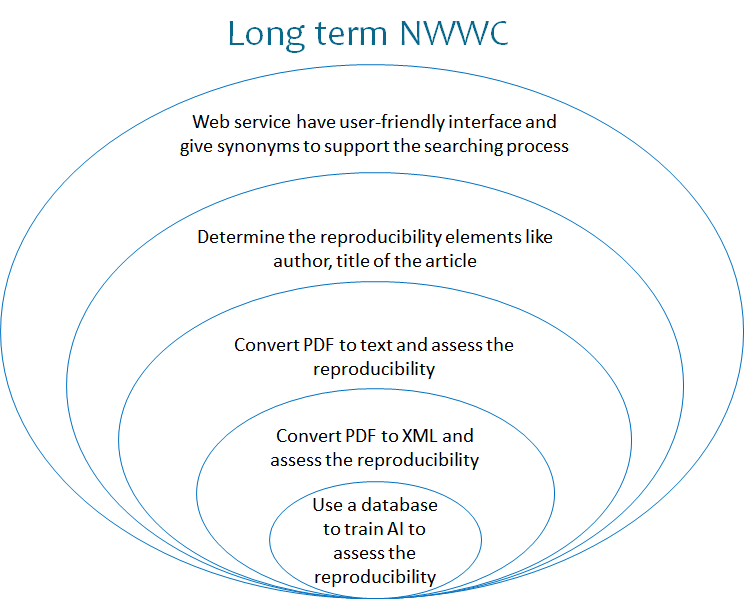
\includegraphics[width = 12cm]{Long_term_NWWC.png}
    \caption{Long term NWWC}
    \label{fig:Long term NWWC}
\end{figure}
\newpage

In the Long-term NWWC Chart, it basicly focus on the user-friendly interface that can support the searching process by giving synonyms, so firstly we need to use database to train model that can assess the reproducibility, next we convert pdf-xml file, after doing the assessment part we need to determine the contributors of reproducibility, then we need feedback and suggestion referent articles to improve our model before it ends to the final part.





%----------------------------------------------------------------------------------------
%	RESULTS AND DISCUSSION
%----------------------------------------------------------------------------------------

\section{Results and Discussion}

\subsection{PDF to XML Development}
% Freshman - Thanh
PDF.co Web API is the flexible Web API that includes a full set of functions from e-signature requests to data extraction, OCR, image recognition, PDF splitting, and PDF splitting. Can also generate barcodes and read barcodes from images, scans, and PDFs.\\
Use from API or via 300+ Integrations: we can use PDF.co from anywhere: programming languages, RPA platforms like UI and Automation Platforms such as Zapier, Integromat, IUPath, RPA apps, SalesForce and many others.
Security: PDF.co API runs on top of the secure and certified Amazon AWS infrastructure. All data transfers are encrypted by SSL/TLS encryption.\\
Asynchronous mode is supported so we can process large files and documents with hundreds of pages in the cloud.\\
The SDK samples displayed below explain how to quickly make your application do PDF to XML API in Python with the help of PDF.co Web API. This Python sample code can be used by copying and pasting it into the project. Once done, just compile our project and click Run. The source code is available in \href{https://github.com/bytescout/pdf-co-api-samples}{here}.\\
To use the API we need to create an API KEY variable that holds the PDF.co API key and it’s passed in the request header for authentication purposes. It can also specify parameters for the source PDF file (SourceFile), Page numbers (Pages) whose data would be converted to XML, Destination location (DestinationFile) where output XML will be stored, etc.\\
% Freshman - Kung
Aspose.PDF Cloud is a complete PDF file processing REST API solution, the choice of many Fortune 100 companies across 114 countries. It enables you to create, convert, split, merge, annotate, sign, stamp, watermark \& protect PDF files on any platform without the installation of any third-party plugin or software. It converts PDF documents to various industry-standard file formats. However,
in this post, we will focus on how to change PDF to XML with Aspose.PDF Cloud SDK for Python. The API is not limited to Python SDK, but SDKs for other popular programming languages are available as well.
and today,XML is the most widely used language for data sharing between humans and computers in this digital era. It provides portable and well-structured information, that makes it easier for applications and devices of all kinds to use, store, transmit, and display data. And in your daily routine, you came across the need to convert different file formats to XML for data sharing or processing.
As you know, PDF is the most reliable file format used to exchange and distribute documents. So in this post, I will give you a walkthrough of how to convert PDF to XML with Python using Aspose.PDF Cloud.

% Freshman - Huy
A web service API for converting pdf to xml is PDF Table.
In order to use PDF Table API, we need to sign up in \href{https://pdftables.com}{PDF Table Homepage} to get the API key.
After that, install pdftables\_api from git by the command
\begin{verbatim}
pip install git+https://github.com/pdftables/python-pdftables-api.git
\end{verbatim}
To convert a PDF file to xml using PDF Table API, you can change the api key, input, output file name in the Python file ``pdftableuser.py''.
The disadvantage of this API is that it is optimized for extracting data from table PDF, so when we test with a paragraph, the performance is not so good.

PDF Miner is a famous Python library to extract text from pdf file.
To install pdfminer library:
\begin{verbatim}
pip install pdfminer
\end{verbatim}
It can convert PDF to TXT file very well. However, when we convert PDF to XML, it reads each character in the paragraph.
Use pdfminer library:
\begin{verbatim}
python pdfmineruser.py -o output.{xml/txt} input.pdf
\end{verbatim}

PDF To Text is a Python library that can convert PDF to TXT file.
However, it doesn't have XML format. To install pdftotext library (Anaconda terminal):\begin{verbatim}
conda install -c conda-forge poppler
pip install pdftotext
\end{verbatim}

% SpinBEC - Jiri
GROBID (GeneRation of BIbliographic Data) is a machine learning library which can extract, 
and re-structure PDF into structured XML/TEI. GROBID can extract metadata from headers or citations. 
Advantage of GROBID is a function to segment the full text of an article to section levels, 
which helps quickly identify a specific part of an article.

CERMINE (Content ExtRactor and MINEr) is an open source system, which extracts data from scientific articles. 
Similarly, to GROBID, CERMINE incorporates documents into metadata. CERMINE surpasses GROBID in all aspects regarding titles, 
abstracts, and references. On certain datasets, CERMINE outperforms GROBID on certain datasets, such as authors and keywords.

PDFMEF (PDF Multi-entity Extraction Framework) is a framework serving for extracting various types of content from technical documents. 
PDFMEF covers content classifiers and extractors as academic paper classifier, PDFBox or pdffigures2 for information extraction. 

SCIENCEPARSE4 is a system for extracting data from raw academics PDFs. It can extract post headers like titles, authors and abstract. 
Moreover, it can extract and analyses citation references and divide articles into sections where each article is with heading and body text.  

\subsection{Assess reproducibility from text}
The simplest way to assess reproducibility is using text file. The main idea of this approach is that we search the related keywords of reproducibility inside the text file obtained after convert the original pdf format.

First, we convert the pdf file given by the user to txt format, using \textbf{pdftotext} Python library.
After that, the document is represented by Bag-of-Words corpus using \textbf{NLTK} Python library, and a \textbf{corpora dictionary} is returned.
Finally, we assess reproducibility with the following search queries:
\begin{itemize}
\item \textbf{Check data availability}:
\begin{verbatim}
(data OR information OR materials OR measurements)
AND (availability OR available)
\end{verbatim}
\item \textbf{Check code availability}:
\begin{verbatim}
(code OR software OR softwares OR artifact)
AND (availability OR available)
\end{verbatim}
\item \textbf{Check method availability}:
\begin{verbatim}
(method OR directions OR process OR procedure OR technique)
AND (availability OR available)
\end{verbatim}
\end{itemize}
\subsection{Assess reproducibility from XML}


% Hehehe, Kung Thanh Alvin Tho write here.
The maximum reproducibility score is 3, which means the article satisfies all 3 criteria: data, code and method availability. The minimum reproducibility score is 0, of course.
The source code to assess reproducibility by text file is provided in \textbf{assess\_txt.py} in the repository \url{https://bitbucket.org/nordlinglab/nordlinglab-reprodm/src/master/flask_docker/flask/assess_txt.py}.

In general, it is not an effective and reliable method to assess reproducibility. We are more interested in xml-based method.\\

P-value algorithm\\
\textbf{Before running (this step should be done offline} \\
1. Collect papers with their label "reproducible / not reproducible"\\
2. Using PDF Miner, and gensim, represent the pdf papers by Bag-of-Word model. (I have done it before).\\
3. Save the Bag-of-Word corpus of all the training papers in a cv file\\
4. Calculate mean frequency of words in dictionary in reproducible set and not reproducible set.\\
5. Find the words that have the most significant difference in mean frequency between the two set. They will be the features. Save the words in a csv file.\\
6. Calculate the total frequency of the selected features in each irreproducible paper, save it in other csv file, maybe sort it to easy using.\\
\textbf{Running (received the input and find p-value)}\\
1. Given a paper, represent it as Bag-of-Word. (I have done it before)\\
2. Find the total frequency of the selected features in the received paper.\\
3. Calculate p-value:\\
$p$ =$ \frac{Number of irreproducible papers has total frequency > received paper}{Total number of irreproducible papers}$\\
4. Small p-value means the received paper is more likely to be reproducible.

Finally, the web service looks like presented in fig \ref{fig:web_service}.

\begin{figure}[h]
    \centering
    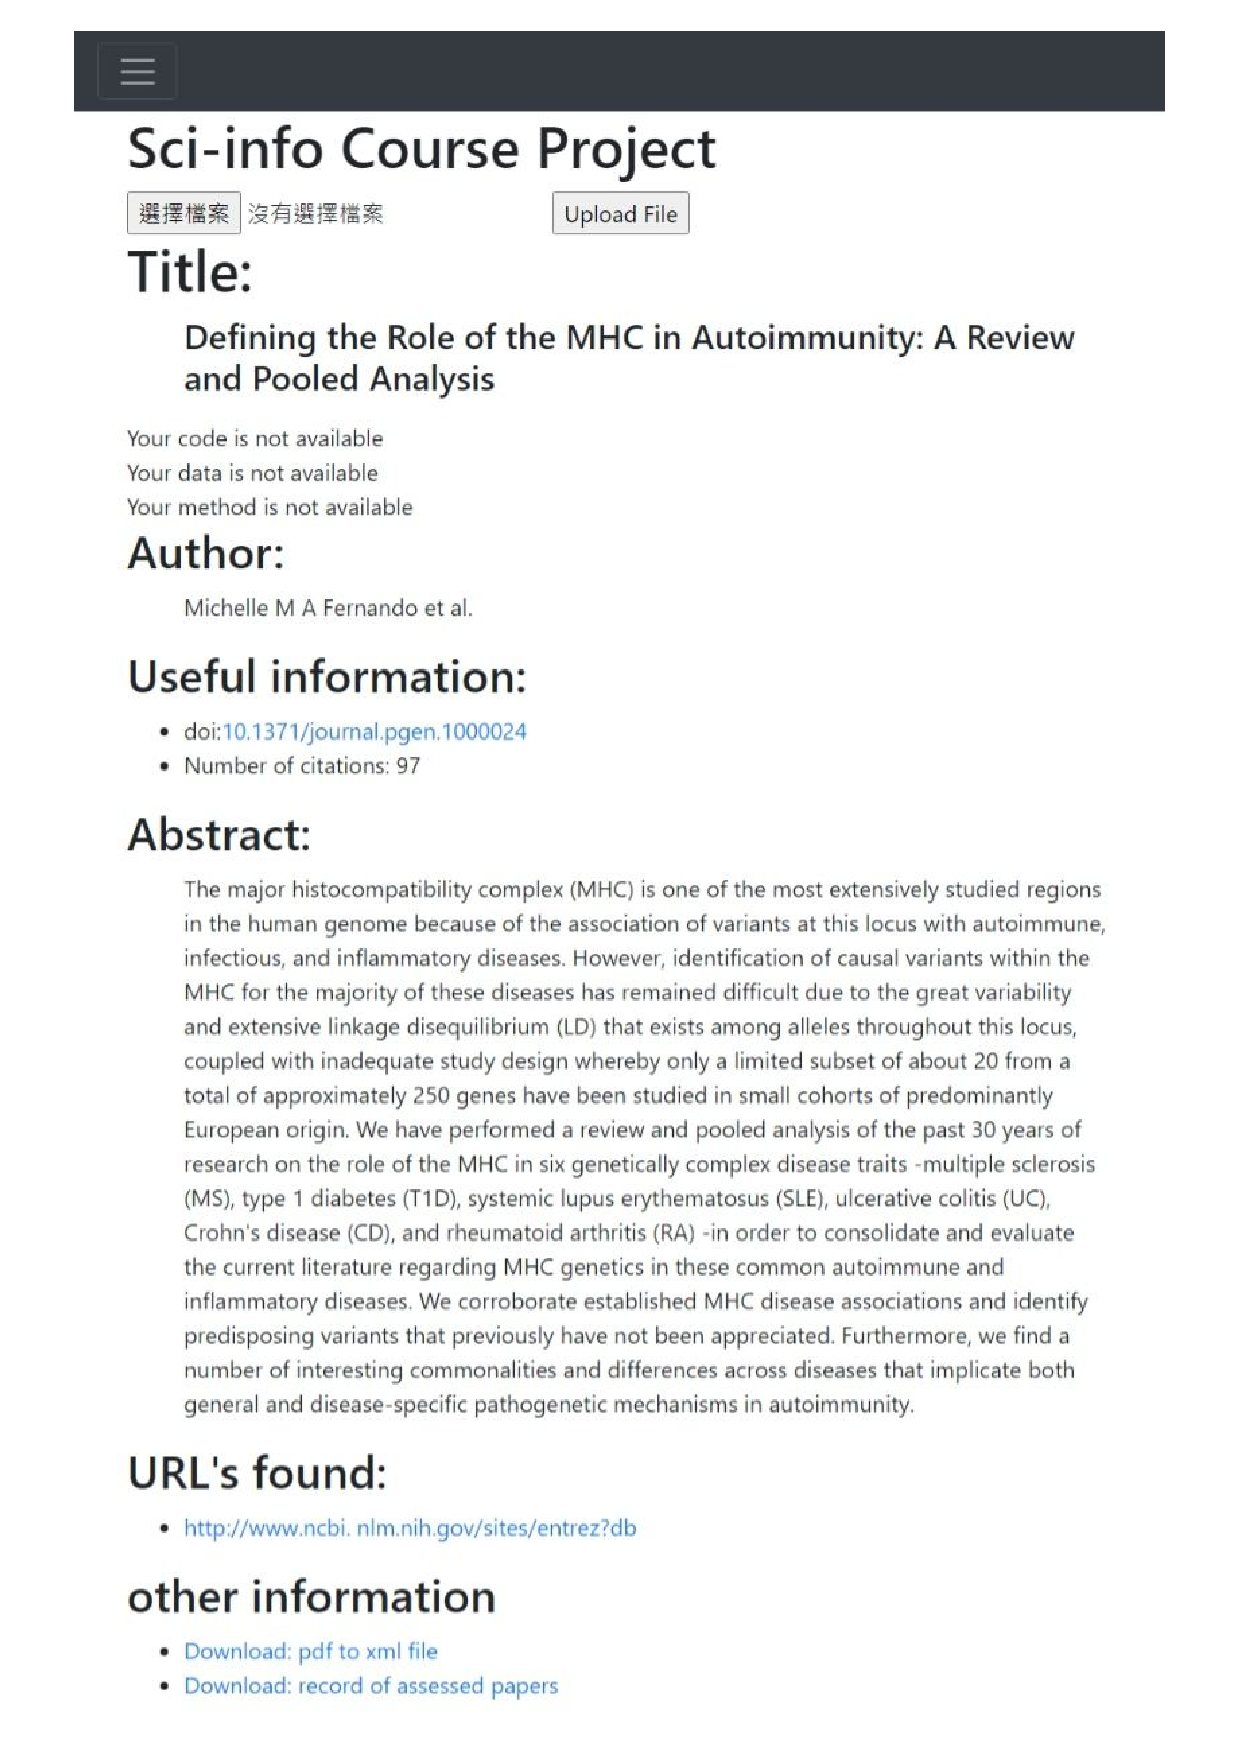
\includegraphics[width = 7cm]{webservice}
    \caption{The web service to extract information from a scientific paper and assess reproducibility}
    \label{fig:web_service}
\end{figure}
\newpage


%----------------------------------------------------------------------------------------
%	CONCLUSION
%----------------------------------------------------------------------------------------
\section {Conclusion}

We began the semester by learning about the importance of reproducibility. Then, by learning how to properly conduct academic research for scientific articles, we began 
this journey of creating a free web service to assess reproducibility. During this process we created a web service that can be fully installed and/or used by anyone. Our 
web service is still at its early stages, but it serves as a foundation for what we hope to do: create a free service so that anyone can assess their scientific articles in a more 
cost and time-effective manner. It has been a great learning experience for us during this process and we hope our project can only help many scientists, engineers and students who are in need 
of a better way to assess reproducibility. 








%----------------------------------------------------------------------------------------
%	BIBLIOGRAPHY
%----------------------------------------------------------------------------------------

\renewcommand{\refname}{\spacedlowsmallcaps{References}} % For modifying the bibliography heading
\bibliographystyle{apalike}
\bibliography{technical_report.bib} % The file containing the bibliography

%----------------------------------------------------------------------------------------

%----------------------------------------------------------------------------------------
%	APPENDIX
%----------------------------------------------------------------------------------------
\appendix

\section{Appendix - Search String} \label{appendix:search_strings}
We started from just throwing words into the search bar at the very beginning, basically copying and pasting words that were provided from the lecture slides and getting hundreds of thousands of hits. Most of them are not relevant. To get the result we wanted, we learned to narrow the search by using search operator like “and”, “and not”, etc. This will help bind the synonyms we were searching for and exclude the articles that had random synonyms scattering inside.
    The result seems to improve as the number of hits dropped to couple thousand as we use “and” to bind more and more words together. But soon after the number drop below 100, we realized that we are also kicking out a lot of relevant articles. Using only “and, and not” will narrow our search too far and just wasn’t an efficient way of picking the right articles.
    Then we tried to use the concept of intersection by expanding the searching string, and then use “and” to include synonym separately. (A OR B OR C ….) AND (X OR Y OR…) AND (M OR N OR…). This will pick out the articles that had the some of the synonym we wanted without demanding them to all exist at the same time. And we applied the same method to different genre of synonym.
The professor told us this is the proper way to search, expand first then narrow and narrow it down.
    At this stage of the search, we were still putting synonyms into the bracket by “feels” and removed the ones we “felt like” didn’t belong. The professor taught us the “and check” to systematically check if the synonyms are helpful. Put an “and” operator at the very back of the search string and put in one keyword at a time, see if that particular word affects the result overall. If the first dozen articles remain irrelevant, remove the word and try out the next one, this should effectively get us the synonyms that “actually matters”. 
    Now that we had a proper collection of synonyms, all we had to do was use the proper search operator to yield the desired result. So, we tried out “title”, it clamped down the search too hard; “abstract”, kind of useless since the search already included it; “W/”, helped a little; “key”, same as “abstract” … the list goes on. 
    After we learned how each operator work on its own, we decided to put them together, using different search method on different parts of the article. We also learned to search in specific subject areas to rule out the unwanted phycology articles.
    We later found out that keyword might appear on certain sections of the article like “abstract” but not in the rest of the article. An ideal relevant hit should have keywords throughout the article, thus we put search operator on each section with different search method and finally we got an accuracy of 60~70%. 
    We’ve learned that it’s really tricky to get the middle sweet spot of the whole search. And I think we’ve made a reasonable cut out of the spectrum.


\subsection{Search String on tools and methods to asses reproducibility in Web of Science}
TI=(method  OR  tool  OR  metric  OR  technique  OR  model ) AND TI=(assess  OR  evaluate  OR  judge  OR  estimate  OR  determine  OR  calculate) AND TI=(reproducibility  OR  repeatability  OR  ( reproducibility  AND  metric )  OR  ( estimate  AND  reproducibility )) AND ALL=(scientific  OR  computational  OR  technical  OR  experimental  OR  ( scientific  AND  research ) ) AND ALL=(work  OR  study)

Number of hits - 55

\subsection{Search String tools and methods to asses reproducibility in Scopus}
( TITLE-ABS-KEY ( method  OR  tool  OR  metric  OR  technique  OR  model )  AND  TITLE ( ( assess  OR  evaluate  OR  judge  OR  estimate  OR  determine  OR  calculate ) )  AND  TITLE ( reproducibility  OR  repeatability  OR  ( reproducibility  AND  metric )  OR  ( estimate  AND  reproducibility ) )  AND  ALL ( scientific  OR  computational  OR  technical  OR  experimental  OR  ( scientific  AND  research ) )  AND  ALL ( work  OR  study )  AND NOT  TITLE-ABS-KEY ( readability  OR  reliability  OR  eligibility  OR  validity ) )  AND  PUBYEAR  >  1999 

Number of hits -> 72

\begin{figure}[h]
    \centering
    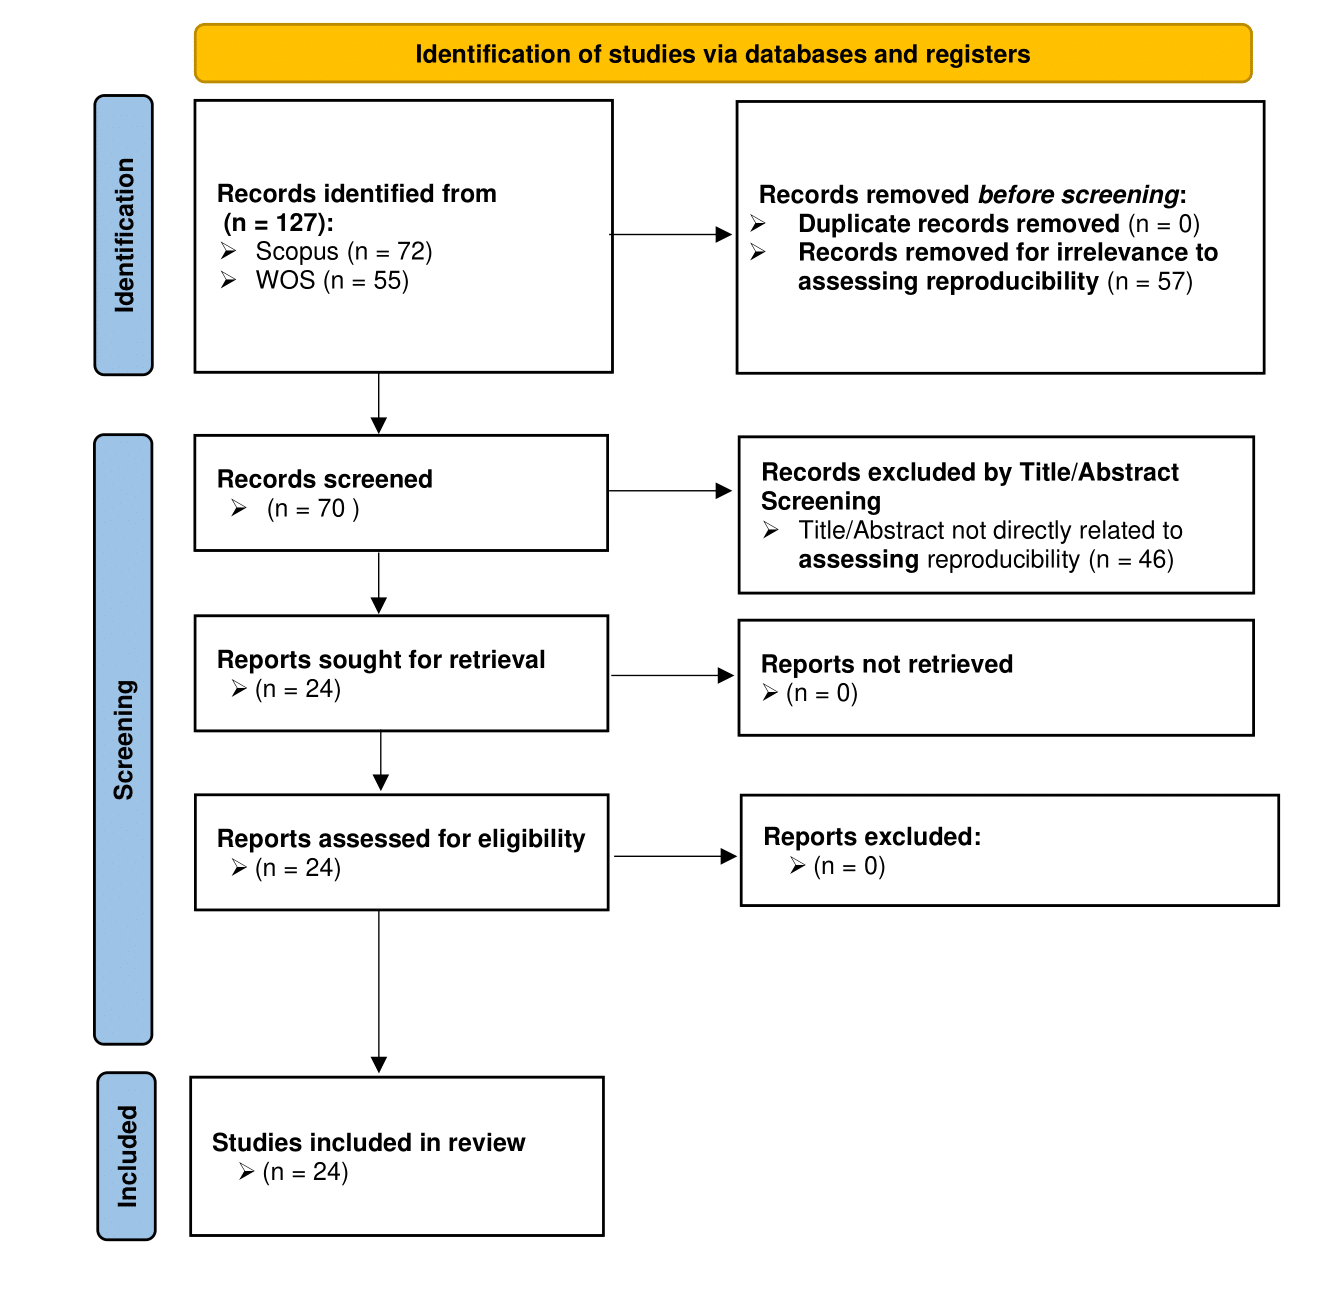
\includegraphics[width = 12cm]{prisma_assessment}
    \caption{PRISMA flow chart for tools and methods to assess reproducibility}
    \label{fig:PRISMA_chart_tools_and_methods_assess_reproducibility}
\end{figure}


\subsection{Search String for Metrics of Assessing reproducibility in Web of Science}
ALL = ((Metric OR standard OR scale) AND (assess OR measure OR estimate OR evaluate OR determine OR calculate OR judge) AND (replicability OR reproducibility) AND (scientific OR technical OR experimental OR computational ) AND (work OR study OR research ) NOT medical NOT medicine NOT chemistry NOT spectroscopy NOT nuclear NOT food NOT biomedical NOT environmental NOT microbiology NOT physics NOT ophthalmology NOT neuroscience NOT radio NOT dentistry NOT oral NOT rehabilitation NOT biochemical NOT biochemistry NOT geochemistry NOT geophysics) and Chemistry Analytical or Biochemical Research Methods or Radiology Nuclear Medicine Medical Imaging or Biotechnology Applied Microbiology or Neurosciences or Spectroscopy or Geochemistry Geophysics or Materials Science Multidisciplinary or Ophthalmology or Physics Applied or Biochemistry Molecular Biology or Food Science Technology or Orthopedics or Pharmacology Pharmacy or Surgery or Clinical Neurology or Sport Sciences or Physiology or Genetics Heredity or Mathematical Computational Biology (Exclude – Web of Science Categories) and Veterinary Sciences or Plant Sciences or Instruments Instrumentation or Meteorology Atmospheric Sciences or Engineering Chemical or Health Care Sciences Services or Engineering Mechanical or Energy Fuels or Environmental Sciences or Geosciences Multidisciplinary or Oncology or Public Environmental Occupational Health or Nursing or Medicine Legal or Rehabilitation or Ecology (Exclude – Web of Science Categories) and Psychiatry or Urology Nephrology or Dermatology or Materials Science Characterization Testing or Cardiac Cardiovascular Systems or Rheumatology or Telecommunications or Medicine General Internal or Acoustics or Biology or Endocrinology Metabolism or Geriatrics Gerontology (Exclude – Web of Science Categories) and Engineering Biomedical or Materials Science Biomaterials or Materials Science Textiles or Medicine Research Experimental or Metallurgy Metallurgical Engineering or Otorhinolaryngology or Agriculture Multidisciplinary or Biophysics or Infectious Diseases or Obstetrics Gynecology (Exclude – Web of Science Categories) and Engineering Electrical Electronic or Physics Multidisciplinary or Agronomy or Anthropology or Automation Control Systems or Dentistry Oral Surgery Medicine or Education Educational Research or Information Science Library Science or Materials Science Ceramics or Pathology (Exclude – Web of Science Categories) and Business or Engineering Industrial or Mechanics or Paleontology or Remote Sensing or Robotics or Chemistry Applied (Exclude – Web of Science Categories) and Psychology Multidisciplinary or Statistics Probability or Psychology Experimental or Nutrition Dietetics or Fisheries or Chemistry Multidisciplinary or Electrochemistry or Hematology or Oceanography or Optics or Peripheral Vascular Disease or Psychology Clinical or Toxicology or Agriculture Dairy Animal Science or Engineering Civil or Psychology Mathematical or Construction Building Technology or Marine Freshwater Biology (Exclude – Web of Science Categories) and Engineering Multidisciplinary or Psychology Applied or Psychology Social or Mathematics Interdisciplinary Applications or Microbiology or Polymer Science or Psychology Developmental or Respiratory System or Virology or Cell Biology or Chemistry Physical or Computer Science Hardware Architecture or Environmental Studies or Geology or History Philosophy Of Science or Horticulture or International Relations or Management (Exclude – Web of Science Categories) and Nanoscience Nanotechnology or Reproductive Biology or Sociology or Soil Science or Zoology or Allergy or Anesthesiology or Archaeology or Astronomy Astrophysics or Behavioral Sciences or Business Finance or Chemistry Inorganic Nuclear or Chemistry Medicinal or Economics or Engineering Aerospace or Engineering Geological or Engineering Manufacturing or Engineering Petroleum (Exclude – Web of Science Categories) and Multidisciplinary Sciences or Family Studies or Forestry or Gastroenterology Hepatology or Geography or Industrial Relations Labor or Law or Materials Science Paper Wood or Mathematics or Mathematics Applied or Medical Laboratory Technology or Microscopy or Mineralogy or Ornithology or Parasitology or Pediatrics or Physics Condensed Matter or Political Science or Psychology Educational (Exclude – Web of Science Categories) and Substance Abuse or Urban Studies (Exclude – Web of Science Categories)

Number of hits -> 30

\begin{figure}[h]
    \centering
    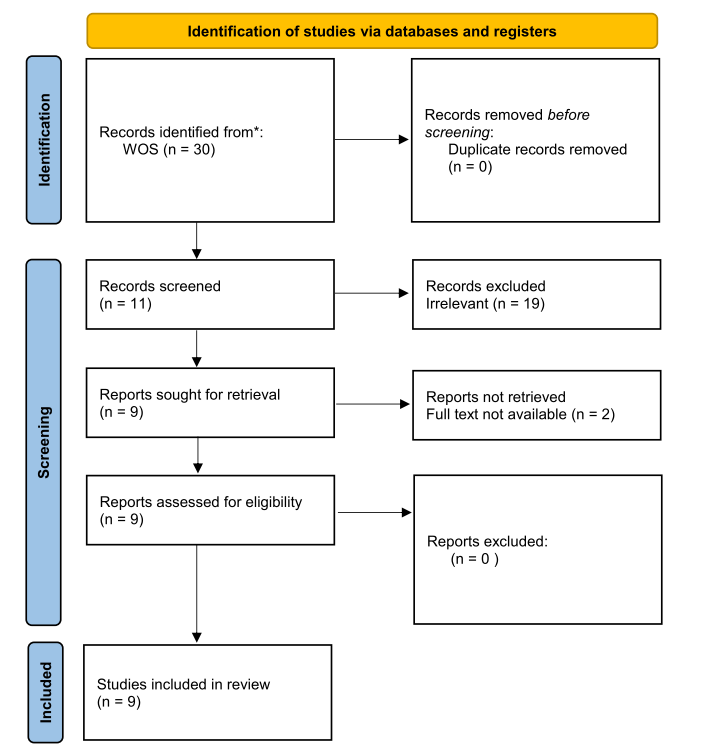
\includegraphics[width = 12cm]{PRISMA_metrics}
    \caption{PRISMA flow chart for the metrics to assess reproducibility}
    \label{fig:PRISMA_chart_metrics_assess_reproducibility}
\end{figure}


\subsection{Search string on studies that attempted to assess reproducibility}
% Search string Tho
To search for papers that assessed reproducibility of other papers, we build the search string:
\begin{quote}
reproducible AND reproducibility AND (replicability OR transparency) AND (research OR scientific OR publication OR investigation OR analysis) AND ("reproducible research" OR "reproducibility study" OR "reproducibility report" OR "reproducibility investigate" OR 
"reproducibility analysis") AND (assess OR evaluate)
\end{quote}

\begin{table}[h]
\centering
\begin{tabular}{|c|clll|}
\hline
Database                		& \multicolumn{4}{c|}{\textbf{Number of article}}           \\ \hline
\textbf{Scopus} 			& \multicolumn{4}{c|}{{\color[HTML]{329A9D} 223 results}} 	\\ \hline
\textbf{Web Of Science} 	& \multicolumn{4}{c|}{{\color[HTML]{329A9D} 23 results}}    \\ \hline
\textbf{Engineering Village}	& \multicolumn{4}{c|}{{\color[HTML]{329A9D} 39 results}}   \\ \hline
\end{tabular}
\caption{This numbers of articles in database}
\label{table1}
\end{table}
% PRISMA (Tho)
First, we recorded search results from Scopus, WOS, and Engineer Village. In the first step, the 24 duplicate records have been removed. In the second step, we erased 221 irrelevant titles and 22 irrelevant abstracts. Continuously, eight articles unavailable to get eligible full-text files have been excluded. Finally, the evaluation result relies on 6 per 10 studies chosen to put into our literature review after removing two weak reproducibility results and two wrong research studies fields. Therefore, it can be clear that the six articles are best to consider within their title, which can appear as references below:

1. "Reproducible Research Practices and Transparency across the Biomedical Literature". Shareen, A. I. et al.

2. "Assessing data availability and research reproducibility in hydrology and water resources". Stagge, J. H. et al.

3. "An empirical analysis of journal policy effectiveness for computational reproducibility". Stodden, V. et al.

4. "Reproducible research and GIScience: an evaluation using AGILE conference papers". Nust, D. et al.

5. "Reproducible research practices are underused in systematic reviews of biomedical interventions". Page, M. J. et al.

6. "Transparency and reproducibility of observational cohort studies using large healthcare databases". Wang, S. V. et al.

\begin{figure}[H]
    \centering
    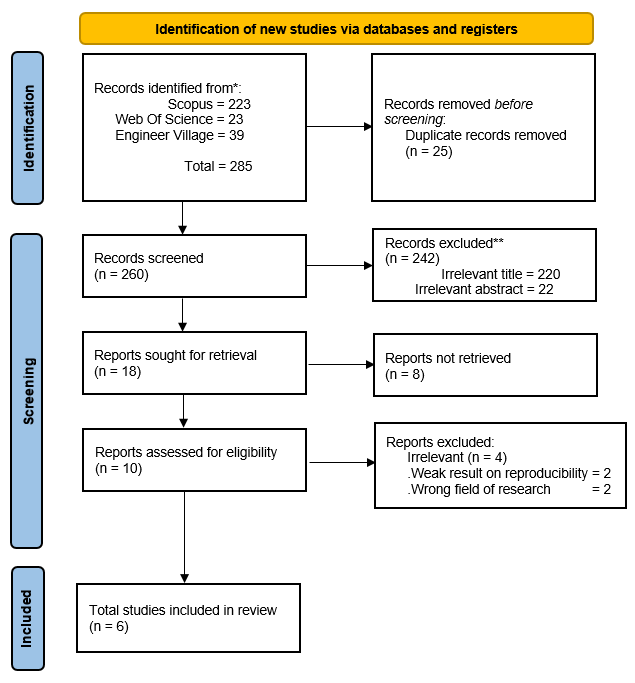
\includegraphics[width = 12cm]{chart.png}
    \caption{PRISMA flow chart for studies that assess reproducibility}
    \label{fig:PRISMA_chart_studies_assess_reproducibility}
\end{figure}
\newpage


\section{Variables used in different metrics to assess reproducibility} \label{appendix:tables_for_metrics_to_assess_reproducibility}
\begin{table}[!htb]
\caption{Variables to measure computational reproducibility}
\centering
\label{table:variables_25}
\begin{tabular}{|p{1.7cm}|p{2.9cm}|p{9cm}|}
\hline
Factors & Methods & Description \\
\hline
Method & Problem statement & Is there an explicit mention of the problem the research seeks to solve? \\
Method & Goal & Is the research goal explicitly mentioned? \\
Method &  Research question & Is there an explicit mention of the research question(s) addressed? \\
Method &  Research method& Is there an explicit mention of the research method used? \\
Method & Algorithm & Is there an explicit mention of the algorithm(s) the research used?  \\
Method & Hypothesis & Is there an explicit mention of the hypotheses being investigated? \\
Method & Prediction &  Is there an explicit mention of prediction related to the hypotheses? \\
Method & Experiment setup & Experiment setup Are the variable settings shared, such as hyperparameters? \\
Method & Contributions & Does the paper state the contributions or implications of the research? \\
Method & Related study & Does the paper explicitly mention related literature? \\
Method & Scope and limitations & Is there an explicit mention of scope and limitations of the research? \\
Method & Machine Learning & Is there an explicit mention of using machine learning for analysis? \\
Method & Statistical analysis & Does the paper conduct any statistical analysis? \\
Method & Conclusion & Is there an explicit outcome concluded in the paper? \\
Data & Model results & Is the output of the model constructed share? \\
Data & Training data & Is the training set shared? \\
Data & Validation data & Is the validation set shared? \\
Data & Testing data & Is the test set shared? \\
Data & Evaluation criteria & Is the evaluation metrics (e.g., Accuracy, R-squared, etc.) of the model shared? \\
Data & Data preprocessing & Is the method of data preprocessing of the analysis shared, including data merging or feature engineering? \\
Data & Publicly available data &  Is the data availiable to public? \\
Data & Time series data &  Does the paper use time series data for analysis (e.g., across multiple years or months)? \\
Data & Data source & Does the paper explicitly state the data source?  \\
Experiment & Method source code & Is the system code available as open source? \\
Experiment & Hardware & Is the software used in the research explicitly mentioned (Python, R, etc.) ?\\
\hline
\end{tabular}
\end{table}


\begin{longtable}[c]{|p{2cm}|p{4cm}|p{8cm}|}

\caption{FEXRep framework 41 variables to measure 
         reproducibility of a scientific work.\label{table:variables_41_FEXREP}}\\

 \hline
 Factors & Methods & Description\\
 \hline
 \endfirsthead

 \multicolumn{3}{c}{FEXRep framework 41 variables to
                    measure reproducibility of a 
                    scientific work. (Cont.\ref{table:variables_41_FEXREP})}\\
 \hline
 Factors & Methods & Description\\
 \hline
 \endhead

 \endhead

 \multicolumn{3}{c}{FEXRep framework 41 variables to
                    measure reproducibility of a 
                    scientific work. (Cont.\ref{table:variables_41_FEXREP})}\\
 \hline
 Factors & Methods & Description\\
 \hline
 \endhead
 
 \hline
 \endfoot
\endlastfoot
Statistical & real\_p & Statistical measurement used to validate a hypothesis against observed data\\
Statistical & real\_p\_sign & The signs parsed from p-value expressions\\
Statistical & p\_val\_range & Difference of the highest and the lowest p-value in the paper\\
Statistical & num\_hypo\_tested & Assume that the number of hypothesis tests is equal to the total number of p-values with test statistics\\
Statistical & extend\_p & A boolean indicating whether the p-value features are associated with a test\\
Statistical & num\_significant & Total number of significant p-values \\
Statistical & sample\_size & Number of participants or observations\\
Bibliometric & num\_citations & Total number of times the target paper is cited since it was published\\
Bibliometric & self\_citations & Self-citation count by excluding references authors by any co-author of the target paper \\
Bibliometric & references\_count & The number of references the target paper cites\\
Bibliometric & normalized\_citations & Average number of citations per year since the target paper is published\\
Bibliometric & citationVelocity & Average of the publication's citations for the last 3 years or less aiming to capture the current popularity and and relevance of work\\
Bibliometric & influentialReferencesCount & Absolute p values\\
Bibliometric & influentialCitationCount & Counts citations in which the paper had a strong impact on the citing work\\
Bibliometric & citations\_next & Measures early citation momentum of a paper by the number of citations in the first 3 years\\
Bibliometric & u\_rank & Calculates the rank of the author's affiliation university, 0-1 if the university ranks in top 100, else it is given the default value 2 \\
Bibliometric & openaccessflag & Weather the paper has open-access or not\\
Bibliometric & age & Number of years since the paper was published\\
Bibliometric & coCite$2$ & The co-citation index between two papers is the number of papers that cite both of them. Gives the number of similar papers within 2 years after the target paper was published\\
Bibliometric & coCite$3$ & Similar to coCIte2 except that it counts similar papers within 3 years after the target paper was published\\
Author & author\_count & Total number of authors of the target paper\\
Author & avg\_pub & Average number of publications of al the authors of the target papers\\
Author & avg\_hidx & The average h-index of all authors of the target paper\\
Author & avg\_high\_inf\_cites & The average number of highly influential citations of all authors\\
Author & avg\_auth\_cites & The average number of citations of all authors\\
Venue & Venue\_CiteScore & A standard to measure citation impact for journals\\
Venue & Venue\_SNIP & The average citation impact of the publications of a journal, using Scopus data\\
Venue & Venue\_Scholarly\_Output & The total count of research outputs, to represent productivity\\
Venue & Venue\_Precent\_Cited & Proportion of documents that have received at least 1 citation\\
Venue & Venue\_Citation\_Count & The number of citations received in one year for the documents published in the previous 3 years\\
Venue & sjr & The average number of weighted citations received in a year divided by the number of documents published in the last 3 years\\
Semantic & citations\_background & Number of times the given paper is cited as background\\
Semantic & citations\_result & Number of times the given paper is cited as result\\
Semantic & reference\_background & References cited in a given paper in background\\
Semantic & reference\_methodology &  References cited in a given paper in methodology\\
Semantic & reference\_result &  References cited in a given paper in result\\
Semantic & upstream\_influential\_me-thodology\_count & The number of papers referenced in the target paper in which the citation context is classified as methodology and the referenced paper was classified as influential \\
Semantic & funded & Acknowledgement of a funding agency\\
Semantic & subject & Serial titles classified into 335 subjects, in Elsevier\\
Semantic & subject\_code & Gives a unique code to the subject\\
 \hline


 \end{longtable}


\end{document}
